% ---------------------------------------------------------------------------
% ---------------------------------------------------------------------------
% Junção de templates encontrados no Overleaf
% facilitando a vida do aluno de pós da UFABC
% Modelo LaTex para preparação do documento final de Dissertação de Mestrado
% ninguém do programa de pós da informação validou se presta
% ---------------------------------------------------------------------------
% ---------------------------------------------------------------------------

\documentclass[
	% -- opções da classe memoir --
	12pt,					% tamanho da fonte
	openright,				% capítulos começam em pág ímpar (insere página vazia caso preciso)
	oneside,					% para impressão em verso e anverso. Oposto a oneside
	a4paper,					% tamanho do papel. 
	% -- opções da classe abntex2 --
	%chapter=TITLE,			% títulos de capítulos convertidos em letras maiúsculas
	%section=TITLE,			% títulos de seções convertidos em letras maiúsculas
	%subsection=TITLE,		% títulos de subseções convertidos em letras maiúsculas
	%subsubsection=TITLE,	% títulos de subsubseções convertidos em letras maiúsculas
	% -- opções do pacote babel --
	english,					% idioma adicional para hifenização
	%french,					% idioma adicional para hifenização
	%spanish,				% idioma adicional para hifenização
	brazilian				% o último idioma é o principal do documento
	]{abntex2}

% ---------------------
% Pacotes OBRIGATÓRIOS
% ---------------------
\usepackage{lmodern}				% Usa a fonte Latin Modern			
\usepackage[T1]{fontenc}			% Selecao de codigos de fonte.
\usepackage[utf8]{inputenc}		% Codificacao do documento (conversão automática dos acentos)
\usepackage{lastpage}			% Usado pela Ficha catalográfica
\usepackage{indentfirst}			% Indenta o primeiro parágrafo de cada seção.
\usepackage{color}				% Controle das cores
\usepackage{graphicx}			% Inclusão de gráficos
\usepackage{caption}
\usepackage{subcaption}
\usepackage{microtype} 			% Melhorias de justificação
% ---------------------
		
% ---------------------
% Pacotes ADICIONAIS
% ---------------------
\usepackage{lipsum}						% Geração de dummy text
\usepackage{amsmath,amssymb,mathrsfs}	% Comandos matemáticos avançados 
\usepackage{setspace}  					% Para permitir espaçamento simples, 1 1/2 e duplo
\usepackage{verbatim}					% Para poder usar o ambiente "comment"
\usepackage{tabularx} 					% Para poder ter tabelas com colunas de largura auto-ajustável
\usepackage{afterpage} 					% Para executar um comando depois do fim da página corrente
\usepackage{url} 						% Para formatar URLs (endereços da Web)
% ---------------------

% ---------------------
% Pacotes de CITAÇÕES
% ---------------------
% \usepackage[brazilian,hyperpageref]{backref}	% Paginas com as citações na bibl
% \usepackage[alf]{abntex2cite}				% Citações padrão ABNT (alfa)
%\usepackage[num]{abntex2cite}				% Citações padrão ABNT (numericas)
% ---------------------
% \usepackage[style=authoryear,backend=biber]{biblatex}
\usepackage{siunitx}
\usepackage[style=abnt, backend=biber]{biblatex}
\addbibresource{bibliografia.bib} % Verifique se o nome do seu arquivo .bib é este
\usepackage{csquotes}
% Configurações de CITAÇÕES para abntex2
\include{extras/conf_citacoes}

% Inclusão de dados para CAPA e FOLHA DE ROSTO (título, autor, orientador, etc.)
% ---
% Informações de dados para CAPA e FOLHA DE ROSTO
% ---
\titulo{Modelagem Dinâmica, Cinemática e Controle de um Sistema Bi-Axial com Antena para Rastreio de Satélite}
\autor{Murilo Valentim Alves}
\local{Santo André - SP}
\data{27 de Julho de 2026}
\orientador{Elvira Rafikova}
\coorientador{Ana Paula Pagotti}
\instituicao{%
  Universidade Federal do ABC -- UFABC
  \par
  Centro de Engenharia, Modelagem e Ciências Sociais Aplicadas 
  \par
  Programa de Graduação em Engenharia
de Instrumentação, Automação e Robótica}
\tipotrabalho{Dissertação (Graduação)}
% O preambulo deve conter o tipo do trabalho, o objetivo,
% o nome da instituição e a área de concentração
\preambulo{\textbf{Dissertação de Graduação} apresentada ao Programa de Graduação em Engenharia de Instrumentação, Automação e Robótica (área de concentração: Sistemas Inteligentes), como parte dos requisitos necessários para a obtenção do Título de Engenheiro em Instrumentação, Automação e Robótica.}
% ---

% Inclui Configurações de aparência do PDF Final
\include{extras/conf_pdf}

% O tamanho da identação do parágrafo é dado por:
\setlength{\parindent}{1.3cm}

% Controle do espaçamento entre um parágrafo e outro:
\setlength{\parskip}{0.2cm}  % tente também \onelineskip

% ---------------------
% Compila o indice
% ---------------------
% \makeindex
% ---------------------


%%%%%%%%%%%%%%%%%%%%%%%%%%%
%%  INICIO DO DOCUMENTO  %%
%%%%%%%%%%%%%%%%%%%%%%%%%%%
\begin{document}

% Retira espaço extra obsoleto entre as frases.
\frenchspacing

% ----------------------------------------------------------
% ELEMENTOS PRÉ-TEXTUAIS (Capa, Resumo, Abstract, etc.)
% ----------------------------------------------------------
\pretextual

% Capa
% ---
% Impressão da Capa
% ---
  \begin{capa}%
    \begin{figure}[h!]%
        \centering%
        
\includegraphics[scale=1.2]{figs/logo.png}%
      \end{figure}%
    \center
	\ABNTEXchapterfont\large{Universidade Federal do ABC \\ Centro de Engenharia, Modelagem e Ciências Sociais Aplicadas \\ Programa de Graduação em Engenharia de Instrumenta{\c c}\~ao, Automação e Robótica}
	%\vspace{1.5cm}

    \vfill
    \ABNTEXchapterfont\bfseries\LARGE\imprimirtitulo
    \vfill

	%\vfill
	\ABNTEXchapterfont\large\imprimirautor
	\vfill
%
	Número de Ordem : XXXX
	
    \large\imprimirlocal, \large\imprimirdata

    \vspace*{1cm}
  \end{capa}
% ---

% Folha de rosto (o * indica que haverá a ficha bibliográfica)
\imprimirfolhaderosto*

% Imprimir Ficha Catalografica
\input{pretextual/catalografica}

% Inserir Folha de Aprovação
\input{pretextual/assinaturas}

% Dedicatória
% \input{pretextual/dedicatoria}

% Agradecimentos
% \input{pretextual/agradecimentos}

% Epígrafe
% \input{pretextual/epigrafe}

% Resumo e Abstract
% ---
% RESUMOS
% ---

% RESUMO em português
\setlength{\absparsep}{18pt} % ajusta o espaçamento dos parágrafos do resumo
\begin{resumo}
  O rastreio contínuo de satélites em órbita baixa (LEO) exige sistemas de apontamento dinâmicos e precisos para mitigar perdas de enlace decorrentes da alta velocidade relativa e da diretividade das antenas.
  Este trabalho apresenta o desenvolvimento, modelagem cinemática, implementação e controle de um sistema de pedestal bi-axial (azimute e elevação) automatizado para o rastreio de satélites e recepção de dados meteorológicos de alta resolução (HRPT) na faixa de 1,7 GHz. A cinemática direta do mecanismo foi formulada via parâmetros de Denavit-Hartenberg (D-H). 
  Para garantir a estabilidade e suavidade da trajetória em tempo real com baixo custo computacional, implementou-se um filtro preditivo $\alpha-\beta-\gamma$ embarcado, cujos parâmetros de suavização foram otimizados via varredura sistemática e validados pelo critério de estabilidade de Jury. A arquitetura de hardware e controle foi estruturada em um microcontrolador dual-core ESP32 sob o sistema operacional FreeRTOS, segregando as tarefas de comunicação TCP/interface LCD e a malha de controle do filtro com acionamento dos motores de passo NEMA 17 via drivers DRV8825. A recepção e filtragem do sinal de radiofrequência foram realizadas por meio de uma antena helicone customizada, aliada a um módulo LNA/filtro SAW e um dispositivo SDR. Os resultados demonstram a funcionalidade mecânica e eletrônica do protótipo de baixo custo, garantindo cobertura hemisférica completa e suavização satisfatória na estimativa de posições orbitais.

  \vspace{\onelineskip}
  \textbf{Palavras-chave}: Rastreio de satélites. Pedestal bi-axial. Cinemática D-H. Filtro $\alpha-\beta-\gamma$. Sistema embarcado. ESP32.
\end{resumo}

% ABSTRACT in english
\begin{resumo}[Abstract]
 \begin{otherlanguage*}{english}
  Continuous tracking of Low-Earth Orbit (LEO) satellites requires dynamic and precise pointing systems to mitigate link losses resulting from high relative velocity and antenna directivity. 
  This work presents the development, kinematic modeling, implementation, and control of an automated bi-axial (azimuth and elevation) pedestal system for satellite tracking and high-resolution meteorological data reception (HRPT) at 1.7 GHz. The direct kinematics of the mechanism was formulated using Denavit-Hartenberg (D-H) parameters. 
  To ensure trajectory stability and smoothness in real-time with low computational overhead, an embedded predictive $\alpha-\beta-\gamma$ filter was implemented, whose smoothing parameters were optimized via grid search and validated using Jury's stability criterion. 
  The hardware and control architecture was structured on a dual-core ESP32 microcontroller running the FreeRTOS real-time operating system, segregating TCP communication and LCD interface tasks from the predictive filter loop and stepper motor driving (NEMA 17 via DRV8825 drivers). 
  Radio frequency signal reception and filtering were accomplished using a custom helicone antenna combined with an LNA/SAW filter module and a Software Defined Radio (SDR). The results demonstrate the mechanical and electronic feasibility of the low-cost prototype, ensuring complete hemispheric coverage and satisfactory smoothing of orbital position estimates.

  \vspace{\onelineskip}
  \textbf{Keywords}: Satellite tracking. Bi-axial pedestal. D-H kinematics. $\alpha-\beta-\gamma$ filter. Embedded system. ESP32.
 \end{otherlanguage*}
\end{resumo}
\newpage

% Lista de ilustrações
\pdfbookmark[0]{\listfigurename}{lof}
\listoffigures*
\cleardoublepage

% Lista de tabelas
\pdfbookmark[0]{\listtablename}{lot}
\listoftables*
\cleardoublepage

% ---
% LISTA DE ABREVIATURAS E SIGLAS
% ---
\begin{siglas}
  \item[ABNT] Associação Brasileira de Normas Técnicas
  \item[D-H] Denavit-Hartenberg
  \item[ESP32] Microcontrolador de Sistema em Chip da Espressif Systems
  \item[FreeRTOS] \textit{Free Real-Time Operating System}
  \item[HRPT] \textit{High Resolution Picture Transmission}
  \item[LCD] \textit{Liquid Crystal Display} (Mostrador de Cristal Líquido)
  \item[LEO] \textit{Low-Earth Orbit} (Órbita Terrestre Baixa)
  \item[LNA] \textit{Low Noise Amplifier} (Amplificador de Baixo Ruído)
  \item[NEMA] \textit{National Electrical Manufacturers Association}
  \item[PWM] \textit{Pulse Width Modulation} (Modulação por Largura de Pulso)
  \item[RF] Radiofrequência
  \item[SAW] \textit{Surface Acoustic Wave} (Onda Acústica de Superfície)
  \item[SDR] \textit{Software Defined Radio} (Rádio Definido por Software)
  \item[TCP] \textit{Transmission Control Protocol}
\end{siglas}

% ---
% LISTA DE SÍMBOLOS
% ---
\begin{simbolos}
  \item[$ \alpha $] Parâmetro de suavização de posição do filtro $\alpha-\beta-\gamma$
  \item[$ \beta $] Parâmetro de suavização de velocidade do filtro $\alpha-\beta-\gamma$
  \item[$ \gamma $] Parâmetro de suavização de aceleração do filtro $\alpha-\beta-\gamma$
  \item[$ \theta_i $] Ângulo da junta articulada $i$ nos parâmetros de Denavit-Hartenberg
  \item[$ d_i $] Deslocamento do elo ao longo do eixo $z_i$ na convenção D-H
  \item[$ a_i $] Comprimento do elo ao longo do eixo $x_i$ na convenção D-H
  \item[$ \alpha_i $] Ângulo de torção do elo no eixo $x_i$ na convenção D-H
  \item[$ f $] Frequência da onda de radiofrequência
  \item[$ T_s $] Período de amostragem do sistema de controle
\end{simbolos}

% Inserir o SUMÁRIO
\pdfbookmark[0]{\contentsname}{toc}
\tableofcontents*
\cleardoublepage

% ----------------------------------------------------------
% ELEMENTOS TEXTUAIS (Capítulos)
% ----------------------------------------------------------
\textual
% Elementos textuais com numeração arábica
\pagenumbering{arabic}
% Reinicia a contagem do número de páginas
\setcounter{page}{1}

% Inclui cada capitulo da Dissertação
% ----------------------------------------------------------
% Introdução 
% Capítulo sem numeração, mas presente no Sumário
% ----------------------------------------------------------

\chapter*[Introdução]{Introdução}
\addcontentsline{toc}{chapter}{Introdução}

Todas as antenas, desde modelos mais simples, possuem direções nas quais elas irradiam seu campo eletromagnético com maior intensidade. Essa característica é conhecida como diretividade. O ganho (capacidade de concentrar energia) da antena também está diretamente relacionado com a diretividade \autocite{Ford2008}. Antenas parabólicas são conhecidas pelo sua alta diretivida e seu alto ganho \autocite{hubregt2014}. Segundo \cite{Ford2008}, essas características são a principal vantagem dessa geometria, sendo excelentes para prover sinal forte e consistente de satélites de órbita baixa (Low-Earth Orbit, ou LEO).

Também, segundo \citeauthor{Ford2008}, a diretividade pode ser uma desvantagem das antenas, pois é necessário manter a antena apontada para o satélite desejado durante todo o momento da comunicação. Para isso, é necessário um sistema automático de apontamento de antena. 


% Introdução antiga, divaga do tema principal
Em 1860, James Maxwell previu a existência de ondas eletromagnéticas em radiofrequência. Em 1886, Hertz criou o primeiro sistema de rádio utilizando dois centelhadores \autocite{fusco2006}. Marconi, então, iniciou seus experimentos na área de telecomunicação em 1899, inventando o campo da comunicação sem fio a longas distâncias \autocite{rochol2018}.

%Nova introdução
No final dos anos 50 e início dos 60, com o advento da corrida espacial, a União Soviética realizou o feito histórico que indicou uma nova era à humanidade. Sputnik 1, o primeiro satélite artificial alcançou órbita e transmitia a todas partes do mundo dois canais de "Radiobaliza" (beacon, em inglês) em \SI{20,005}{\mega\hertz} e \SI{40,002}{\mega\hertz} \autocite{Ford2008}. Segundo \cite{Ford2008}, os radios amadores estavam entre os únicos meios de notícias sobre a nave revolucionária (tradução livre).
Atualmente, na camada LEO, existe o lançamento de milhares de satélites da nova constelação da Starlink, além de outras constelações já planejadas para cobrir boa parte da Terra, com um satélite em horizonte local em poucos minutos \autocite{app12199505}.

O apontamento automático de antenas é utilizado para diversas aplicações. A principal funcionalidade desse mecanismo é a de obter uma conexão estável com qualquer equipamento desejado. Para o caso de radioamadorismo, seriam os satélites de órbita baixa \autocite{Ford2008}.
Atualmente, esse sistema é utilizado em antenas é a de obter comunicação de fragatas e navios em alto mar, pois o acesso por solo é impossível \autocite{ueba2016}.
(TODO:  Explicar o que é pedestal de antena)

- como está o panorama de pesquisa atual tipo o que é mais recente de publicação 
 %Feito na seção "estado da arte"

O objetivo desse trabalho está em desenvolver a modelagem dinâmica e cinemática de um sistema pedestal biaxial, criando um protótipo funcional e aplicando os conceitos de controle para a obtenção de imagens meteorológicas vindas de satélites de órbita baixa.

 


% \section*{Figuras}\label{sec:figuras}
% \addcontentsline{toc}{section}{figuras}

% % As normas da~\citeonline[3.1-3.2]{NBR6028:2003} especificam que o caption da figura deve vir abaixo da mesma.

% A Figura~\ref{fig:log} ilustra...

% \begin{figure}[htpb]
%    \centering
%    
\includegraphics[scale=.3]{figs/logo}
%    \caption{Breve explicação sobre a figura. Deve vir abaixo da mesma.}
%    \label{fig:log}
% \end{figure}

% \section*{Tabelas}\label{sec:tabelas}
% \addcontentsline{toc}{section}{tabelas}

% A Tabela~\ref{tab:tabela} apresenta os resultados...

% \begin{table}[htpb]
%    \centering
%    \caption{Breve explicação sobre a tabela. Deve vir acima da mesma.}\label{tab:tabela}
%    \begin{tabular}{|l|c|c|c|c|c|c|r|}
%         \hline
%         \small{XX} & \small{FF} & \small{PP} & \small{YY} & \small{Yr} & \small{xY} & \small{Yx} & \small{ZZ} \\ \hline
%                615 &    18      &     2558   &    0,9930  &    0,9930  &    0,9930  &    0,9930  &    0,9930  \\ \hline
%                615 &    18      &     2558   &    0,9930  &    0,9930  &    0,9930  &    0,9930  &    0,9930  \\ \hline
%                615 &    18      &     2558   &    0,9930  &    0,9930  &    0,9930  &    0,9930  &    0,9930  \\ \hline
%                615 &    18      &     2558   &    0,9930  &    0,9930  &    0,9930  &    0,9930  &    0,9930  \\ \hline
%                615 &    18      &     2558   &    0,9930  &    0,9930  &    0,9930  &    0,9930  &    0,9930  \\ \hline
%    \end{tabular}
% \end{table}

% \section*{Motivação}\label{sec:motivacao}
% \addcontentsline{toc}{section}{Motivação}

% \lipsum[35]

% \section*{Objetivos}\label{sec:objetivos}
% \addcontentsline{toc}{section}{Objetivos}

% \lipsum[36]


% \chapter{Estado da Arte}\label{cap:estArte}

A principal aplicação de sistemas de rastreio automático está relacionada a veículos aéreos não tripulados (VANTs, ou UAVs em inglês), com o intuito de aumentar a distância de operação com relação à base em solo \cite{nugroho2018} \cite{kim2023}.Para rastreio de satélites, existem diversos trabalhos focados em modelar o funcionamento de antenas baseadas em barcos e navios \cite{wang2016} \cite{ueba2016} \cite{gholamiomali2024}. 

\section*{Trabalhos Relacionados a Isto}\label{sec:primTrab}
\addcontentsline{toc}{section}{Trabalhos Relacionados a Isto}

\lipsum[34-36]


\chapter{Objetivos}\label{cap:obj}

O objetivo desse trabalho é desenvolver o protótipo de um sistema de alinhamento automático
de antena helicoidal impressa em impressora 3D. Esse protótipo contará com um sistema de controle motorizado e uma integração com sistemas externos,
como aplicativo de rastreamento de satélites.


\section{Objetivos Especificos}\label{sec:esp}
\subsection{Modelagem e Prototipagem}\label{sec:mod}
A fim de obter êxito no rastreio do sinal enviado pelos satélites, .
Primeiramente, será necessária uma modelagem dos ângulos e os modelos para permitir o cálculo da cinemática
direta do mecanismo e permitir o apontamento do sistema.

\subsection{Sistema de Controle}\label{sec:ctr}
Após a modelagem do sistema, será necessário calcular a resposta do sistema a
estímulos e estabilizar o controle do mecanismo. O sistema de controle utilizado será de
malha aberta, utilizando motores de passo para realizar o controle do mecanismo do sistema.
O sistema de controle deve ser estável e responsivo para acompanhar a trajetória do veículo selecionado. 
Além disso, será utilizado um filtro $\alpha-\beta-\gamma$ para permitir um rastreio 

\subsection{Características Mecâncias}\label{sec:ssb}
O mecanismo deverá possuir duas características principais: velocidade e precisão.
O primeiro fator está relacionado com a resposta do sistema à tarefa. Uma passagem de satélites
de órbita baixa é marcada por momentos de aceleração e desaceleração. O protótipo deverá ser capaz de
efetuar o apontamento da antena em todas as direções de uma semiesfera e ser sensível o suficiente para ter a precisão de
apontamento necessária para a comunicação.

\subsection{Interface com Sistemas Externos}
Diversos aplicativos, programas e bancos de dados, disponíveis na internet, fornecem informações sobre órbitas e mudanças de posição
de satélites. O envio desses parâmetros acontece por uma comunicação TCP (Transmission Control Protocol), pelo qual o
sistema irá receber ângulos de azimute e elevação para o apontamento da antena e irá retornar os dados de sua posição atual. Dessa forma, o protótipo deverá ser capaz de
receber e enviar parâmetros para realizar a comunicação com aplicativos e programas.
\chapter{Referencial Teórico}\label{cap:teo}
\section{Referencial e Rastreio de Satélites}\label{sec:ground_tracking}
Para iniciar a modelagem do sistema, é necessário descrever o referencial e entender como a estação de solo e o satélite se localizam no espaço.
Segundo \cite{soler1994}, utilizando um modelo esférico aproximado da Terra \ref{fig:modelagem_ang_visada} e sabendo a localização de latitude $\phi_S$ e longitude $\lambda_S$ da antena na estação, é possível estipular a direção em azimute e elevação para o apontamento da antena.
O raio da Terra para o modelo esférico será considerado de $R=6371 km$ e a distância do satélite em relação ao centro do modelo será considerada como $r = R+h$, com $h$ sendo a altitude de sua órbita.
Pode-se obter a longitude $\lambda_S$ na qual o vetor $\vec{r}$ intercepta a superfície da Terra, sendo possível traçar um triângulo reto esférico e utilizar a lei de Napier para obter a relação $\cos\gamma=\cos\phi_S\cos(\lambda_S-\lambda)$ \cite{soler1994}. Dessa forma, a distância entre o satélite e a estação de solo é dada pela equação \cite{soler1994}:
\begin{equation}
d = r[1+(R/r)^2-2(R/r)\cos\gamma]
\end{equation}
\begin{figure}[ht]
    \centering
    \caption{Modelagem matemática do ângulo de visada}
    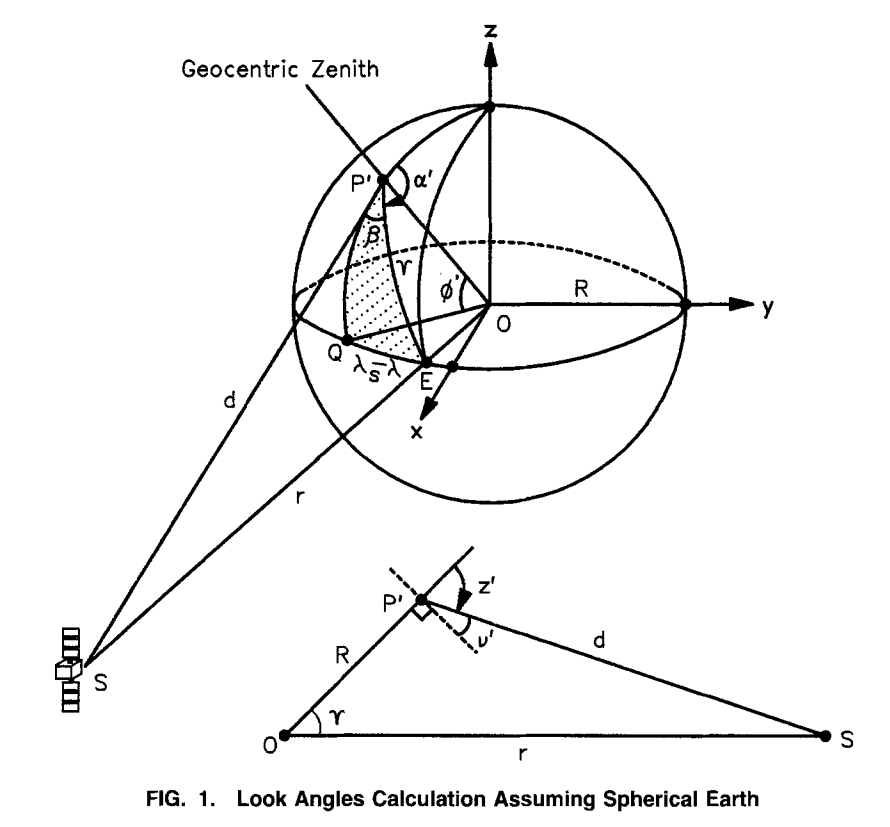
\includegraphics[width=0.8\textwidth]{figs/Interpretacao_geodesica.png}
    \legend{Fonte: \cite{soler1994}.}
    \label{fig:modelagem_ang_visada}
\end{figure}
A partir da equação anterior, é possível calcular a elevação $\nu_S$ e o azimute $\beta_S$ do satélite em relação à estação de solo a partir das seguintes equações:
\begin{align}
\nu_S = \arccos[(r/d)sin\gamma] \\
\beta_S = \arccos(\cot\gamma\tan\phi_S)
\end{align}
Essa modelagem foi feita considerando uma Terra esférica. Na realidade, a Terra possui uma forma aproximada de um elipsoide de revolução. Embora o modelo esférico ofereça uma aproximação inicial simples, ele introduz erros no cálculo do ângulo de elevação (ou distância zenital).
O formato faz com que o modelo esférico tenha algumas discrepâncias com as posições reais. No entanto, como o escopo do trabalho não é o modelo da Terra, mas sim o sistema de controle de apontamento da antena, bastará dizer que há a dedução de na literatura de \cite{soler1994} caso necessária a consulta.
Além disso, é esperado que os aplicativos com os quais o equipamento irá comunicar sejam baseados nos modelos mais completos, enviando a posição de azimute e elevação correta para o alinhamento com o satélite.

Podemos descrever o mecanismo apontamento da antena do pedestal a partir de dois movimentos independentes ortogonais, sendo um de azimute e um de elevação (sendo essa a configuração mais comum para mecanismos de apontamento).
O espaço de trabalho necessário para o acompanhamento contínuo de passagens de satélites corresponde ao hemisfério superior delimitado pelo horizonte local do plano tangente à estação de solo encontrado a 0$^\circ$ de elevação.
Para cobrir integralmente essa semi-esfera, o mecanismo deve ser capaz de efetuar uma rotação completa de $0$ até $2\pi$ (0$^\circ$ até 360$^\circ$) em azimute e uma articulação de $0$ até $\frac{\pi}{2}$ (0$^\circ$ até 90$^\circ$) na elevação.
Embora existam diversos mecanismos que tenham seu ângulo de elevação encurtado, já que em baixas elevações há a obstrução de relevo, estruturas ou atmosfera, o mecanismo desenvolvido nesse trabalho garantirá a varredura de toda região angular teórica.

É importante salientar que a partir das próximas modelagens as variáveis $\theta$ e $\phi$ serão também utilizadas ao se referir ao azimute e à elevação do mecanismo da antena.

\section{Modelagem do Pedestal}\label{sec:modelagem_pedestal}
Segundo \citeauthor{Ford2008}, o sistema pode ser modelado utilizando como base um manipulador esférico de dois graus de liberdade.
Utilizando o modelo pela figura \ref{fig:pedestal}, e utilizando como referência a modelagem de \cite{Bien2021} o ponto fixo que dará a referência do mecanismo com o solo será o da base, dado pelo referencial de coordenadas $O_0$, com versores $[x_0,y_0,z_0]$.
\begin{figure}[ht]
    \centering
    \caption{Modelo de pedestal com controle em azimute e elevação}
    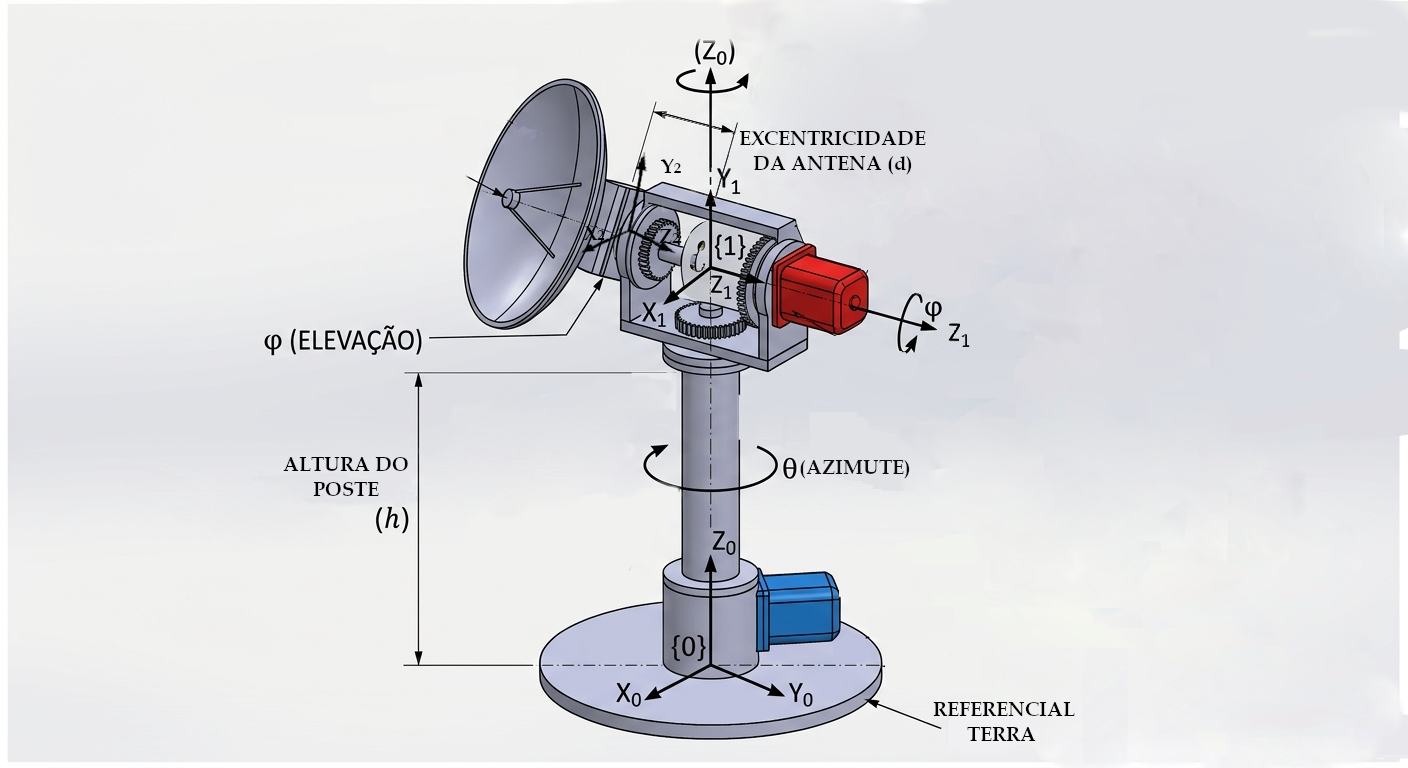
\includegraphics[width=0.8\textwidth]{figs/pedestal_proxy.png}
    \legend{Fonte: Elaborado pelo autor (2026).}
    \label{fig:pedestal}
\end{figure}
(TODO: explicar a localização dos motores)
Um motor é ligado por uma polia à base da antena, permitindo a rotação em torno do eixo Z. O ângulo de rotação do azimute é dado por $\theta$.
O segundo motor está localizado na região na qual a antena se encaixa ao poste do pedestal e é ligado ao eixo da elevação também através do mecanismo de polia. A junção da polia movida com o eixo da elevação tem coordenadas dadas pela origem $O_1$ ($[x_1,y_1,z_1]$) e distância da base dada pelo valor "h".
Além dos referenciais motorizados, será utilizando mais um referencial para descrever a excentricidade da antena, dado por $O_2$ ($[x_2,y_2,z_2]$) e distância de excentricidade "d"; e a região mais extrema que representa a ponta da antena, encontrada em  $O_3$ ($[x_3,y_3,z_3]$) e distância de braço "l".
O modelo da cinemática direta do sistema pode ser obtido a partir dos parâmetros de Denavit-Hatemberg (D-H). Utilizando como referenciais $O_i$ descrita pelos versores de referencial $[x_i,y_i,z_i]$ obtendo a tabela \ref{tab:params_d_h}
\begin{table}[ht]
\centering
\begin{tabular}{rrrrr}
    \hline
    Parâmetro & $\theta_i$ & $d_i$ & $a_i$ & $\alpha_i$ \\
    \hline
    $O_0O_1$ & $\theta$ & h & 0 & frac{$\pi$}{2} \\
    $O_1O_2$ & $\phi$ & -d & 0 & 0 \\
    $O_2O_3$ & 0 & 0 & l & 0 \\
\end{tabular}
\caption{Tabela de parâmetros D-H para o sistema}
\label{tab:params_d_h}
\end{table}

A partir da tabela D-H, a cinemática do sistema está completamente descrita e é possível determinar as matrizes de transformação homogênea de cada ponto utilizando o parâmetro \citeauthor{Siciliano2008}.
\begin{equation}
A^{i-1}_{i} = \begin{bmatrix}
\cos \theta_i & -\sin \theta_i \cos \alpha_i & \sin \theta_i \sin \alpha_i & a_i \cos \theta_i \\
\sin \theta_i & \cos \theta_i \cos \alpha_i & -\cos \theta_i \sin \alpha_i & a_i \sin \theta_i \\
0 & \sin \alpha_i & \cos \alpha_i & d_i \\
0 & 0 & 0 & 1
\end{bmatrix}
\end{equation}
Assim, é possível calcular como referenciais intermediários os seguintes pontos:
\begin{equation}
A^{0}_{1} = \begin{bmatrix}
\cos \theta & 0 & \sin \theta & 0 \\
\sin \theta & 0 & -\cos \theta & 0 \\
0 & 1 & 0 & h \\
0 & 0 & 0 & 1
\end{bmatrix}
\end{equation}
\begin{equation}
A^{1}_{2} = \begin{bmatrix}
\cos \phi & -\sin \phi & 0 & 0 \\
\sin \phi & \cos \phi & 0 & 0 \\
0 & 0 & 1 & -d \\
0 & 0 & 0 & 1
\end{bmatrix}
\end{equation}
\begin{equation}
A^{2}_{3} = \begin{bmatrix}
1 & 0 & 0 & l \\
0 & 1 & 0 & 0 \\
0 & 0 & 1 & 0 \\
0 & 0 & 0 & 1
\end{bmatrix}
\end{equation}
Utilizando a dedução de \cite{Siciliano2008}, pode-se computar a transformação homogênea de estado $T_{i}^{0} = A_{i}^{i-1} A_{i-1}^{i-2}(...)A_{1}^{0}$.
\begin{equation}
T^{0}_{1} = \begin{bmatrix}
\cos \theta & 0 & \sin \theta & 0 \\
\sin \theta & 0 & -\cos \theta & 0 \\
0 & 1 & 0 & h \\
0 & 0 & 0 & 1
\end{bmatrix}
\end{equation}
\begin{equation}
T^{0}_{2} = \begin{bmatrix}
\cos\theta\cos\phi - \sin\theta\sin\phi & -\cos\theta\sin\phi & \cos\theta\sin\phi+\sin\theta\cos\phi & \sin\theta(-\sin\phi) \\
\cos\theta\sin\phi + \sin\theta\cos\phi & \cos\theta\cos\phi & \sin\theta\sin\phi-\cos\theta\cos\phi & \sin\theta\cos\phi \\
0 & 1 & 0 & h-d \\
0 & 0 & 0 & 1
\end{bmatrix}
\end{equation}
\begin{equation}
T^{0}_{3} = \begin{bmatrix}
\cos\theta\cos\phi - \sin\theta\sin\phi & -\cos\theta\sin\phi & \cos\theta\sin\phi+\sin\theta\cos\phi & l-\sin\theta\sin\phi \\
\cos\theta\sin\phi + \sin\theta\cos\phi & \cos\theta\cos\phi & \sin\theta\sin\phi-\cos\theta\cos\phi & \sin\theta\cos\phi \\
0 & 1 & 0 & h-d \\
0 & 0 & 0 & 1
\end{bmatrix}
\end{equation}

\section{Estimação e Rastreio de Satélites}\label{sec:estimation}
Segundo a explicação de \cite{Ford2008}, cada satélite possui um número de catalogação que é utilizada para registrar informações básicas sobre a espaçonave. Embora algumas identificações (como nome e código de catalogação) são inalteradas durante sua vida útil, informações de órbita devem ser atualizadas constantemente por serem dinâmicas.
Agências como a North American Aerospace Defense Command (NORAD) e a National Aeronautics and Space Administration (NASA) utilizam radares e outras formas de medição para determinar a posição e órbita exata de satélites, mantendo um rastreio completo do céu.
Entre as métricas obtidas das observações estão os conhecidos elementos keplerianos. Esses elementos são informações como inclinação, excentricidade, decaimento de órbita, e perigeu.
A partir dos keplerianos, é possível estipular a posição do satélite no espaço em relação a um determinado tempo (passado ou futuro).
Softwares utilizam dessas informações para determinar passagens de diversos satélites e verificar quando estarão acima do horizonte, além de determinar o azimute e a elevação que a antena da estação de solo deverá ter para estar apontada para o satélite.
Apesar de possuir a posição (quase) exata dos satélites, os softwares de rastreio de satélites normalmente não têm uma taxa muito alta de atualização de envio de dados alta, sendo necessário um algoritmo para manter o rastreio durante os pontos sem informações novas.

Existem várias técnicas para a estimação da posição de um satélite ao longo do tempo. A primeira e mais simples é de enviar ao controlador dos motores a posição recebida do aplicativo e replicá-la na antena. O problema com esse método é que a estrutura sofre saltos grandes de posição, além de que a posição da antena ficará estática se o rotor perder a conexão com o software de rastreio.
Uma outra técnica é utilizar um filtro Kalman, que possui camadas de previsão e correção recursiva para fazer com que o Mínimo Erro Quadrático Médio seja nulo em relação a um modelo inicial. E o problema com o Filtro Kalman para esse caso é que ele é relativamente exigente em quesitos de processos, já que precisa recorrentemente atualizar as matrizes de ganhos.
Como é desejado que o projeto funcione completamente embarcado em um microcontrolador, esse tempo maior de processo pode causar demora no controle dos motores e fazer o sistema perder o rastreio do satélite. 

\chapter{Metodologia}\label{cap:metod}
\section{Software de Rastreio e Decodificação}\label{sec:software}
\begin{figure}[h]
    \centering
    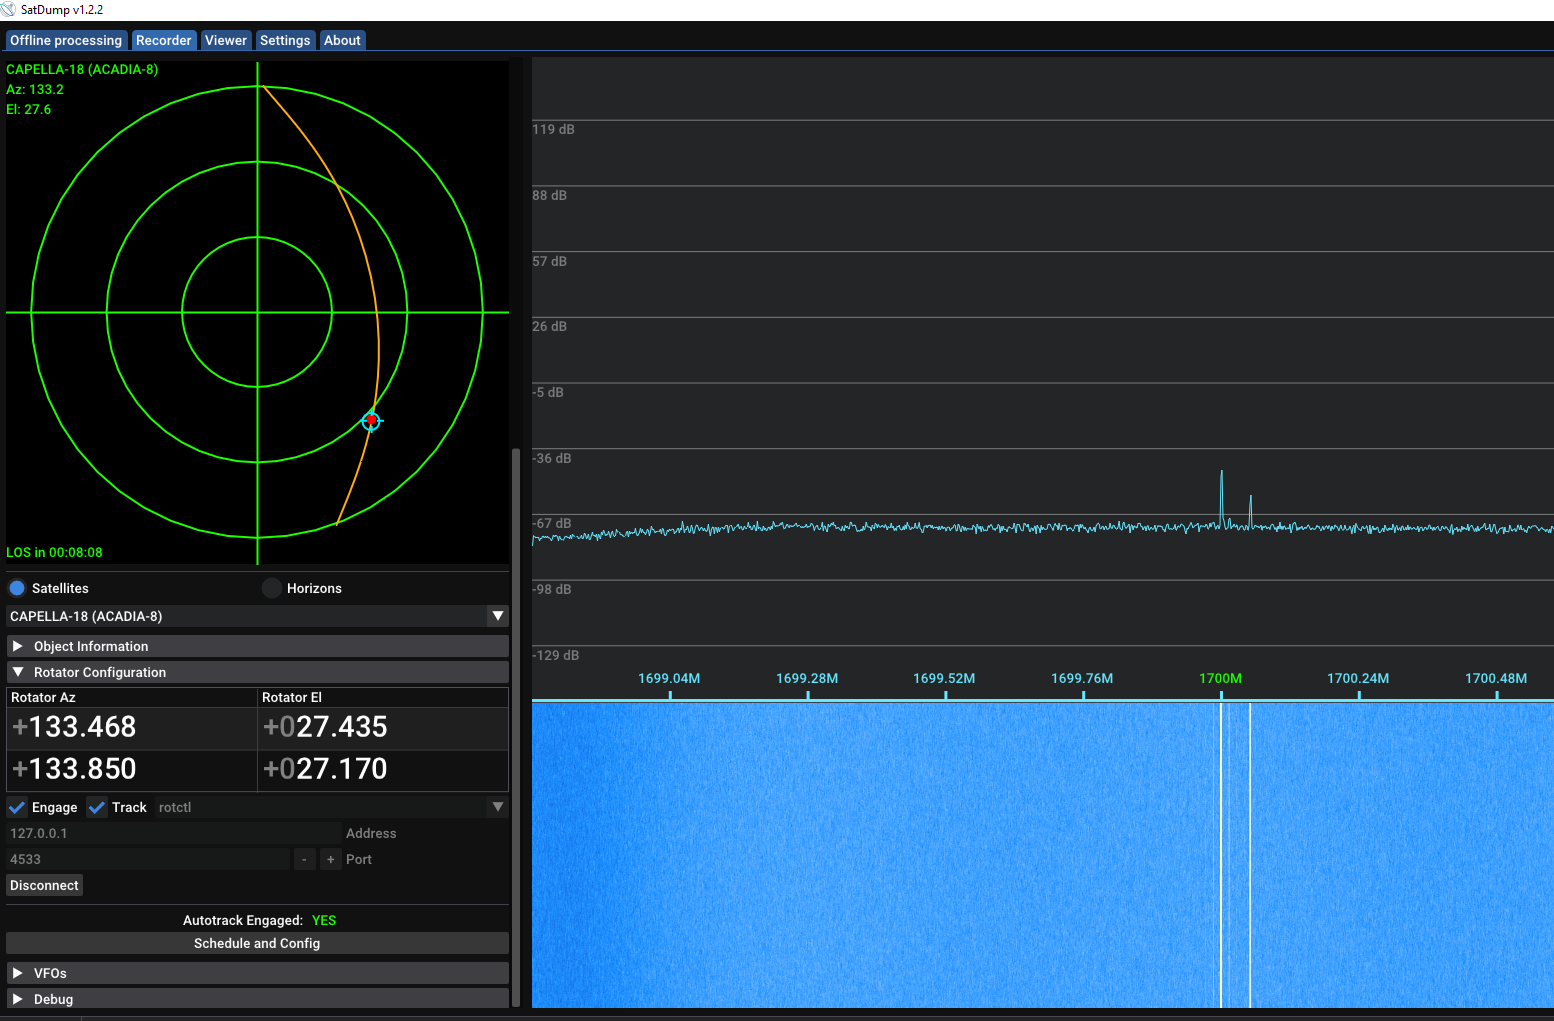
\includegraphics[width=0.8\textwidth]{figs/satdump_example.png}
    \caption{Interface do software SatDump}
    \caption*{Fonte: Autor(2026)}
    \label{fig:satdump}
\end{figure}
O aplicativo de rastreio de satélites principal do trabalho será o SatDump.
Esse programa será utilizado porque ele possui um conglomerado de ferramentas para permitir o rastreio de satélites e a decodificação dos sinais recebidos pela antena da estação de solo.
Na figura \ref{fig:satdump}, é possível observar a interface do Software. O software está dividido em duas partes principais: a painel de controle/rastreio (à esquerda) e o analisador de espectro/cachoeira RF (à direita).

Na região esquerda, existe uma roda polar no topo, que indica algumas informações sobre o satélite rasteado. O texto acima da roda indica o satélite que está sendo rastreado (no caso, o CAPELLA-18), além de suas informações de azimute e elevação.
Abaixo do texto, está a roda polar de fato. A roda polar é uma representação bidimensional de 360° de toda a abóbada celeste visível a partir da localização da estação em solo. O centro do círculo, onde há a intersecção dos eixos, representa o Zênite (elevação de $90^{\circ}$), enquanto os círculos concêntricos indicam as elevações intermediárias de $0^{\circ}$, $30^{\circ}$ e $60^{\circ}$ (do mais externo para o mais interno).
A cruz interna representa a direção cardeal, ou seja, em qual direção do horizonte a antena deve apontar. A seção superior da cruz indica $0/360^{\circ}$, representando o Norte, e o ângulo de azimute é crescente no sentido horário. Desta forma, a linha direita indica $90^{\circ}$ (Leste), a linha inferior indica $180^{\circ}$ (Sul), e a linha esquerda indica $270^{\circ}$ (Oeste).
A linha amarela representa todo o arco que o satélite faz durante essa passagem. O ponto vermelho indica a posição real do satélite. O ícone de mira azul indica a posição que foi passada ao rotor da antena, enquanto o círculo azul representa a posição que o rotor acusa estar.
Mais abaixo há um texto com a informação de tempo estimado até ocorrer a LOS (Loss of signal, ou perda de sinal) do satélite quando este se encontrar abaixo do horizonte.
Na seção de nome "Rotator Configuration" (configuração de rotor), esta área está destinada à conexão do programa com o rotor. Os números de azimute e elevação de da linha superior é a posição teórica onde o satélite está, calculada com base nas informações de órbita e a posição da estação de solo.
A linha inferior indica a posição real de apontamento da antena indicada pelo rotor. Abaixo disso, há a configuração do servidor de controle dos rotores, na qual estão configurados o endereço de IP e a porta para a comunicação. Além disso, existem as opções de "Engage" (engajar), que inicia a conexão com servidor, e "Track" (rastrear), que envia posições atualizadas ao mecanismo de apontamento.

A região direita é dedicada ao processamento e à representação visual do sinal de radiofrequência (RF) recebido pelo aplicativo. Este painel fornece diagnóstico em tempo real da qualidade do enlace de comunicação e é composto por dois elementos gráficos fundamentais alinhados no domínio da frequência: o Analisador de Espectro e o Exibidor em Cachoeira (Waterfall).
O gráfico superior exibe a densidade de potência do sinal capturado em função da frequência, calculada por meio da Transformada Rápida de Fourier (FFT). Seu eixo vertical representa a amplitude (em \text{dB}, decibel) do sinal recebido para cada frequência, enquanto o eixo horizontal indica a frequência em $\text{MHz}$.
O gráfico inferior é conhecido como visualizador em cachoeira representa a variação observada no gráfico acima em função do tempo (eixo y). Esse visualizador é atualizado com as informações mais novas sendo inseridas em cima e as mais antigas "deslizando" para regiões mais abaixo. Esse gráfico é mapeado por cores, nos quais cores próximas ao azul indicam uma intensidade baixa, enquanto cores próximas ao vermelho indicam uma maior intensidade de sinal recebida.
Em geral, essa interface é utilizada para garantir a estabilidade da transmissão durante a passagem, além de permitir observar variações na largura do sinal ou desvios na frequência central da linha ao longo do rastreio.

\section{Motores de Passo}\label{sec:motor_passo}
O sistema de controle da antena será baseado em um pedestal convencional
controlado por dois parâmetros ortogonais principais, sendo estes: azimute e elevação.
Para efetuar o controle desses fatores em uma antena, serão necessários dois motores que atuarão modificando
os ângulos mencionados anteriormente. Como discutido na seção \ref{sec:ground_tracking}, o controle do azimute será feito por 360 graus, enquanto o
controle de elevação atuará somente em 90 graus. Desta maneira, o ângulo de visada total do mecanismo
será dado por uma meia-esfera superior. Essa geometria é considerada suficiente para a detecção e o rastreio de qualquer satélite necessário pela estação de solo.

Os motores de passo utilizados no trabalho são de classe NEMA (National Electrical Manufacturers Association, Associação Nacional de Fabricantes de Equipamentos Elétricos), que padroniza as dimensões e as características de motores em geral. O modelo selecionado é o motor de passo 17HS4401, da classe NEMA 17.
Ele possui ângulo de passo de $1.8^{\circ}\pm5\%$, torque de $4,2\text{kgf}\cdot\text{cm}$, e corrente por fase de $1,5A$.
\begin{figure}[h]
    \centering
    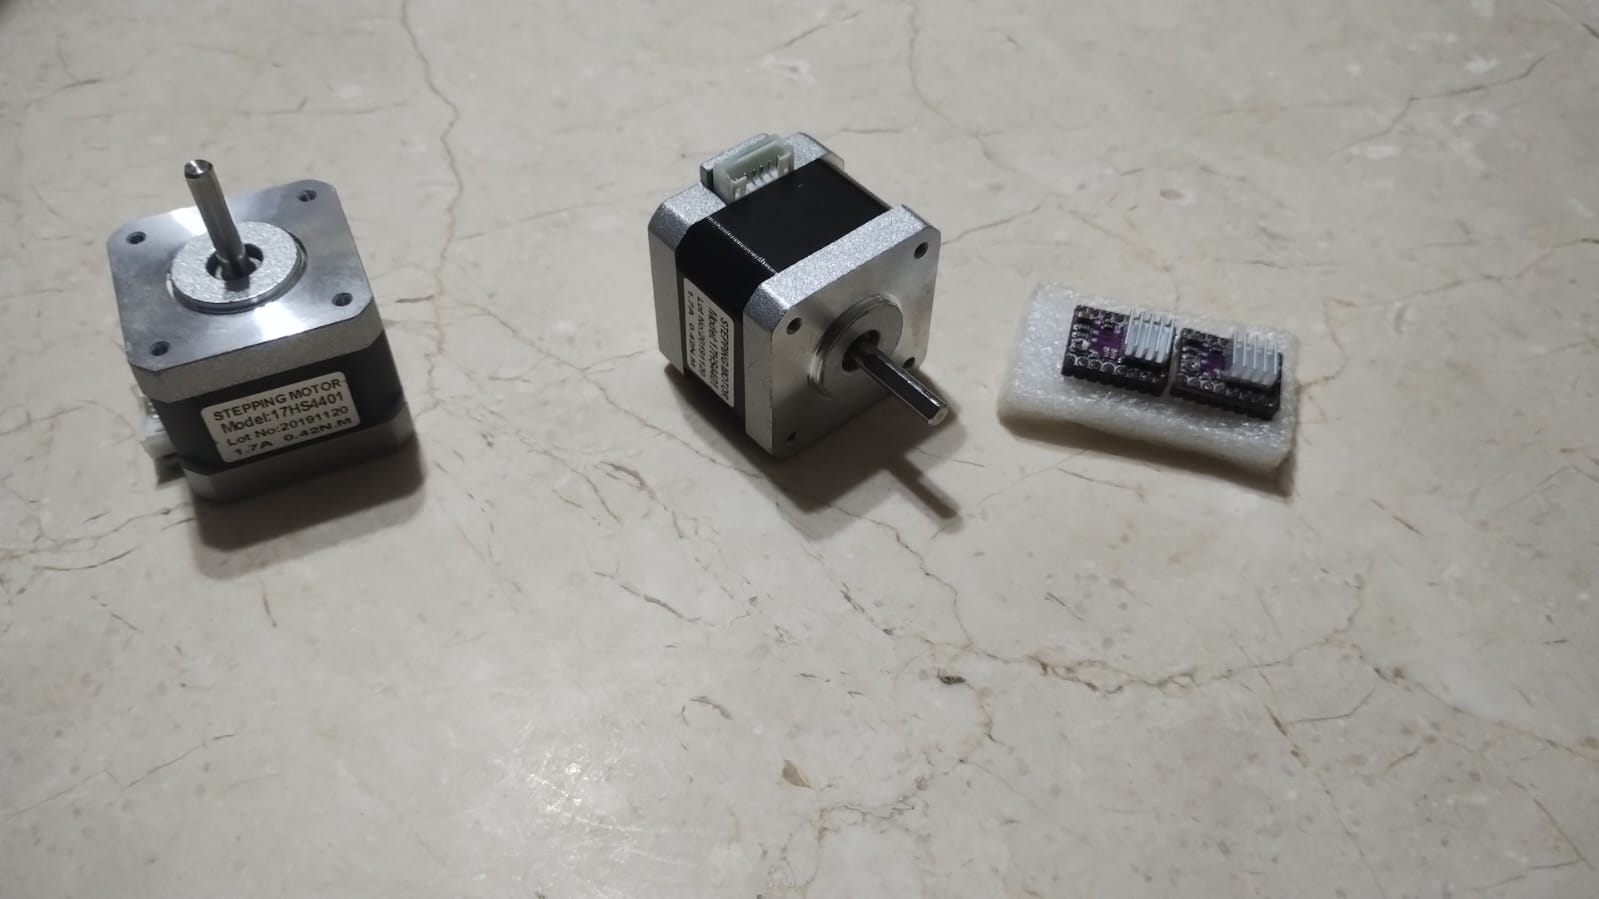
\includegraphics[width=0.8\textwidth]{figs/motores_drivers.jpeg}
    \caption{Motores 17HS4401 e drivers DRV8825}
    \caption*{Fonte: Autor(2026)}
    \label{fig:motores_drivers}
\end{figure}

Para o acionamento dos motores, serão utilizados drivers dedicados DRV8825, configurados para conseguirem atingir a resolução de $1/32$ passo, permitindo elevar a resolução angular teórica de acionamento dos motores para $0,05625^\circ$ por micropasso.
A calibração da posição inicial (homing) das eixos de azimute e elevação será realizada por meio de sensores ópticos, que serão desenvolvidos a partir de LDRs e LEDs. O controlador fará uma varredura para verificar quando o LDR receberá a maior intensidade luminosa. Esse valor máximo indicará o zero do azimute e da elevação.
O acoplamento entre o eixo dos motores e a estrutura da antena será feito utilizando um sistema de redução por correias GT2 de relação 2:1, fazendo com que a resolução real na estrutura seja metade da resolução angular desenvolvida pelo motor.

\begin{figure}[h]
    \centering
    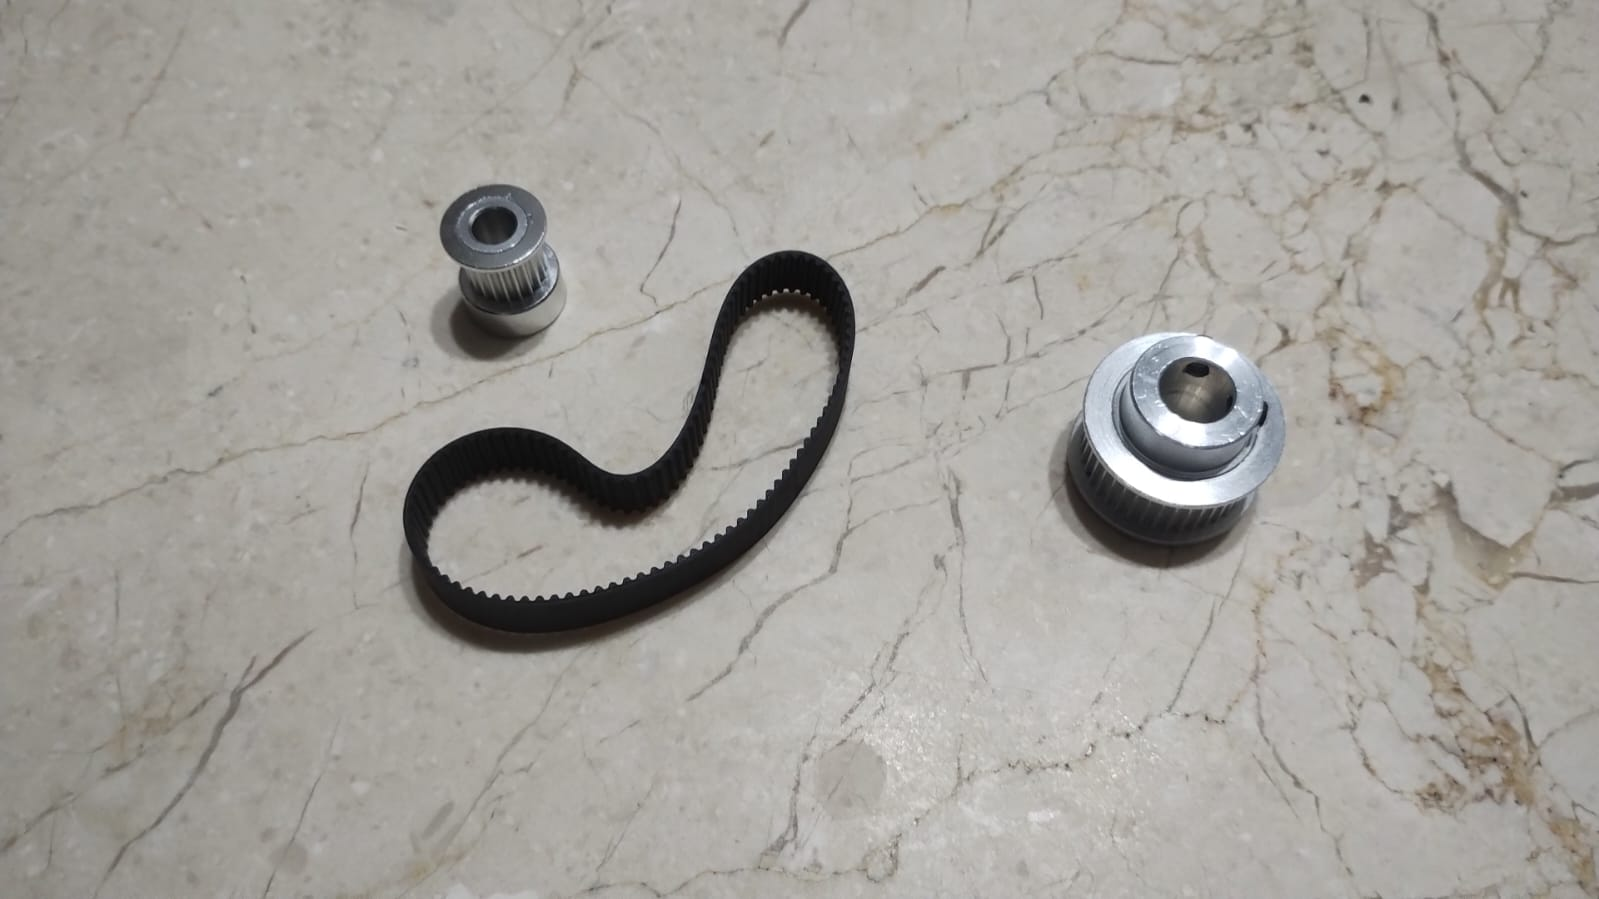
\includegraphics[width=0.8\textwidth]{figs/polias_cinto.jpeg}
    \caption{Polias GT2 com 20 e 40 dentes, além de cinto de 200mm}
    \caption*{Fonte: Autor(2026)}
    \label{fig:polias_cinto}
\end{figure}

\section{Sistema de Comunicação}\label{sec:sistema_comunicacao}
Para o recebimento do sinal de satélite, será utilizando um rádio definido por software (Software Defined Radio, ou SDR), de modelo RTL-SDR V4. Esse dispositivo é capaz de ser programado via software para sintonizar com diversas frequências sem modificação de hardware, tornando-o extremamente versátil para receber comunicação de diversos satélites.
O modelo em questão é capaz de operar em frequências de \SI{500}{\kilo\hertz} a \SI{1766}{\mega\hertz}. Além disso, há um circuito Bias-Tee interno ativável por software, que é capaz de fornecer uma tensão contínua de 4,5 V no conector SMA para alimentação de pré-amplificadores localizados na linha de transmissão utilizando o mesmo cabo coaxial por onde o sinal é recebido.

Devido à extrema atenuação sofrida pelos sinais emitidos pelos satélites ao se propagarem através da atmosfera até a antena de recepção, será utilizado um módulo pré-amplificador e filtrador Nooelec SAWBird+ GOES.
O módulo é composto por dois estágios de amplificação de baixo ruído (LNA) em cascata com um filtro de Onda Acústica de Superfície (SAW) intercalado. Esses compontentes são responsáveis por tratar, filtrar e amplificar os sinais recebidos pela antena.
O conjunto apresenta frequência central em aproximadamente \SI{1688}{\mega\hertz}, com banda passante ajustada para a recepção de \SI{1694,1}{\mega\hertz} e ganho típico de 35 dB, reduzindo interferências de sinais fora da faixa de interesse e compensando as perdas de transmissão.

Todo o sistema será montado dentro do cabo da antena e haverá um cabo extensor USB de \SI{2}{\meter} para realizar a conexão com o computador. O sistema de recepção está representado na figura \ref{fig:sistema_coms}.

\begin{figure}[h]
    \centering
    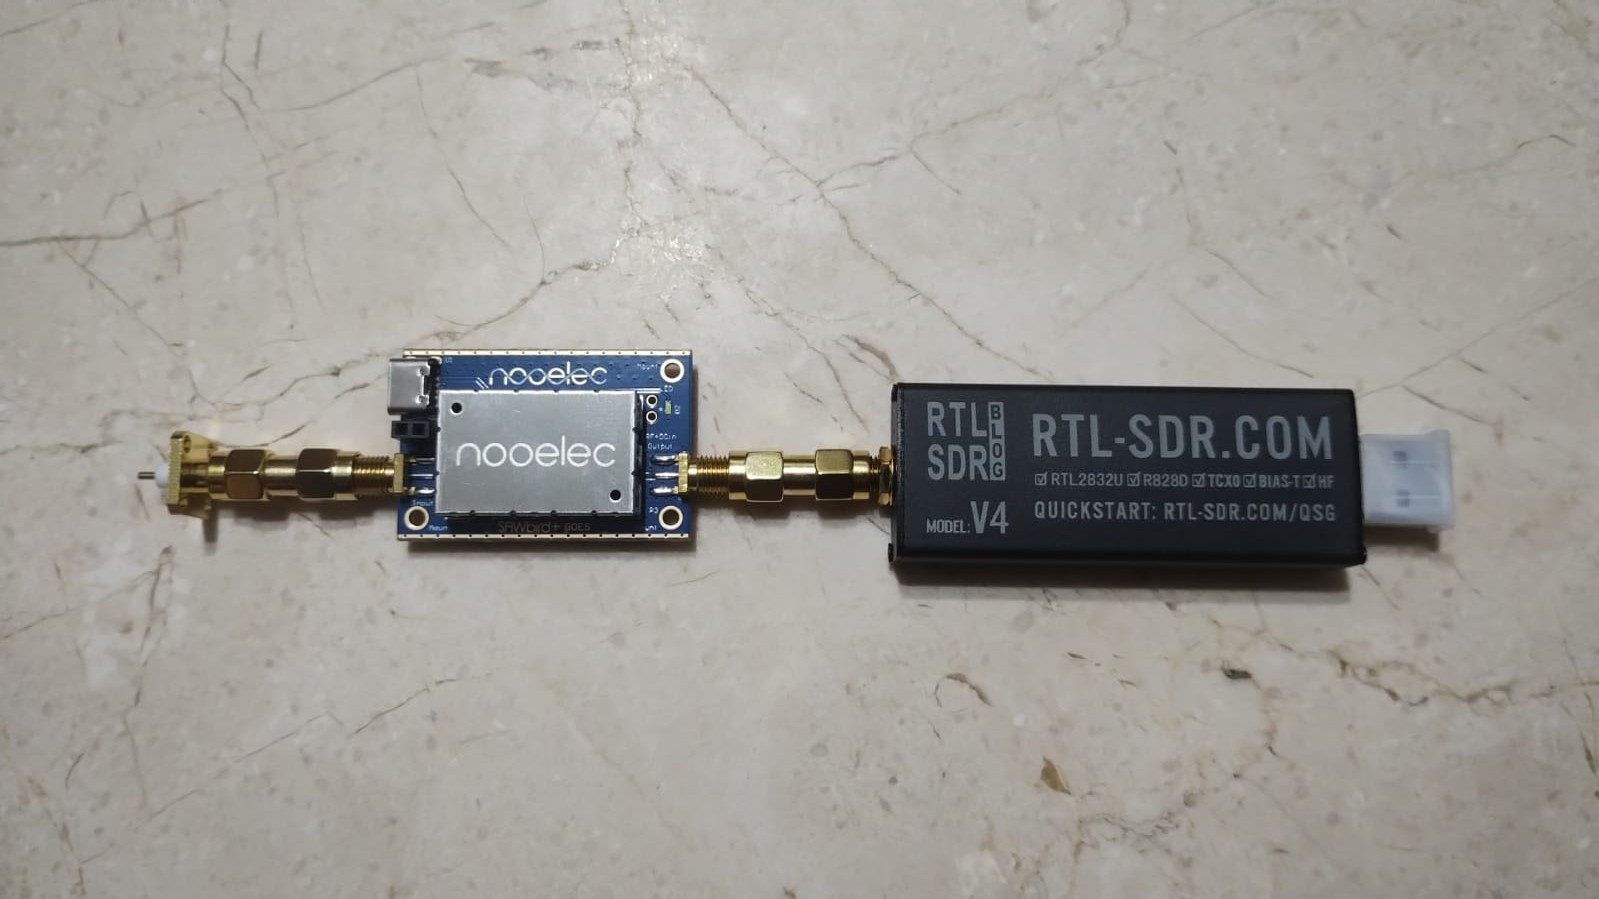
\includegraphics[width=0.8\textwidth]{figs/sistema_comunicacao.jpeg}
    \caption{Sistema de comunicação com ponto de alimentação da antena (dourado) à esquerda, filtro Nooelec (azul) ao centro e SDR (preto) à direita}
    \caption*{Fonte: Autor(2026)}
    \label{fig:sistema_coms}
\end{figure}

\section{Antena}\label{sec:antena}

\begin{figure}[h]
    \centering
    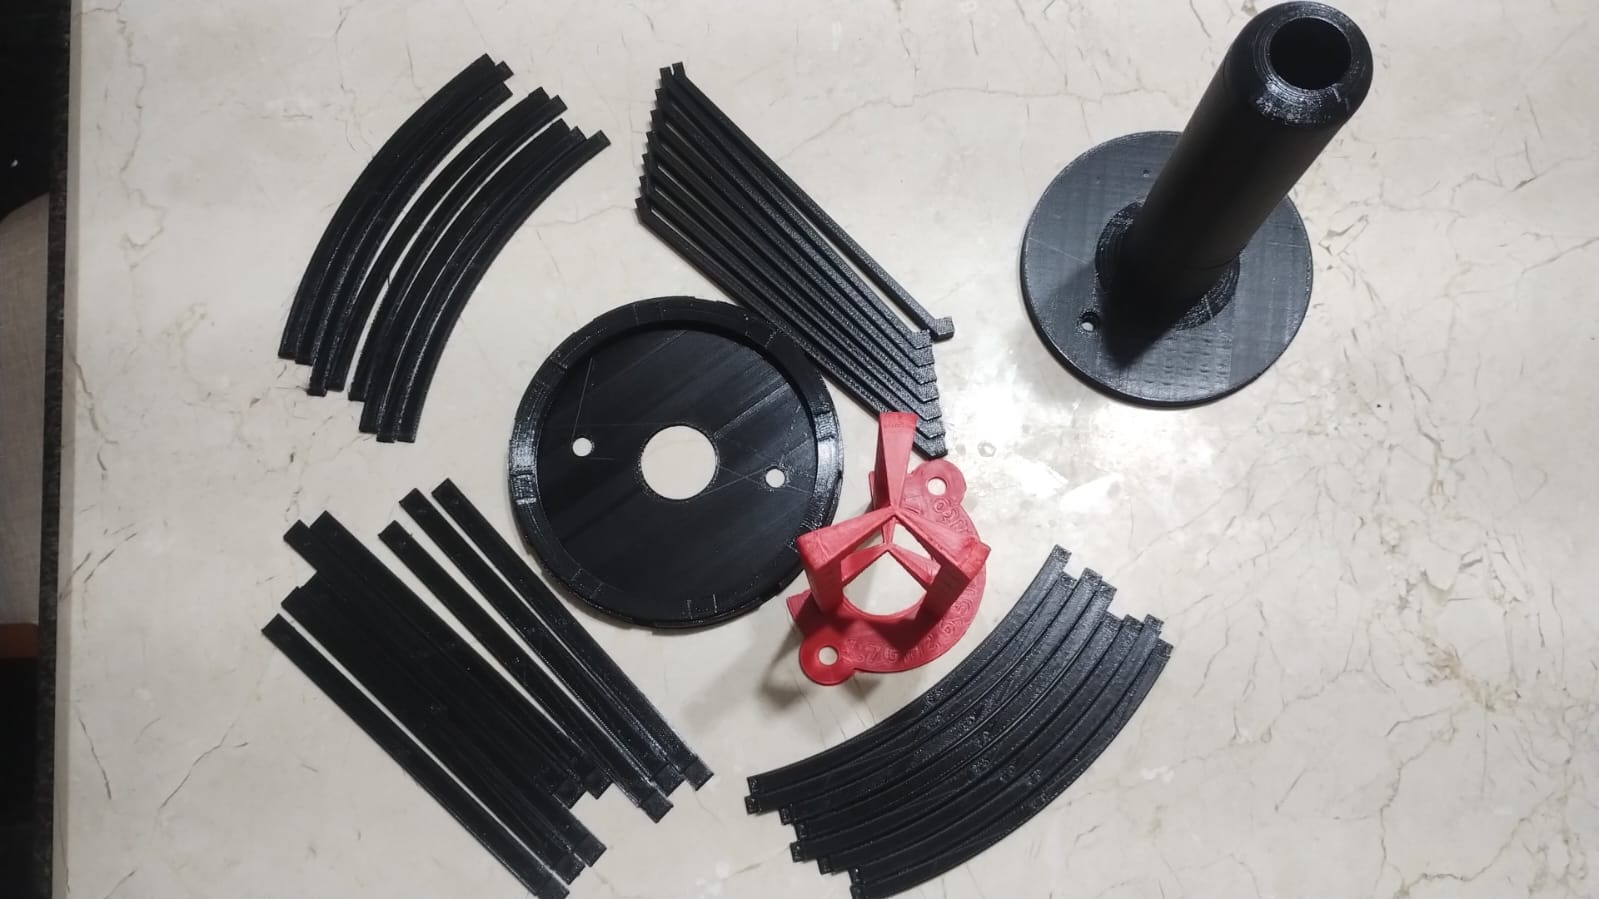
\includegraphics[width=0.8\textwidth]{figs/antena_peças.jpeg}
    \caption{Sistema de comunicação com ponto de alimentação da antena (dourado) à esquerda, filtro Nooelec (azul) ao centro e SDR (preto) à direita}
    \caption*{Fonte: Autor(2026)}
    \label{fig:pecas_antena}
\end{figure}

A antena apresentada no projeto de \cite{tonito2024} é uma Antena Helicone projetada especificamente para a recepção de sinais de alta resolução de satélites meteorológicos na faixa de 1,7 GHz, desenvolvida para a captura de imagens enviadas no modo HRPT (High Resolution Picture Transmission).
Este modelo combina a simplicidade construtiva com características eletromagnéticas de alto ganho e alta diretividade, sendo ideal tanto para uso  montado no sistema de rastreio automatizado desenvolvido nessa tese.
A antena helicone é uma variação da antena helicoidal no modo axial combinada com um plano Terra (ground plane) levemente cônico.

Satélites que transmitem em HRPT operam com Polarização Circular (normalmente RHCP — Right-Hand Circular Polarization).
Uma antena com hélice helicoidal garante o casamento de polarização correto com a onda incidente, evitando perdas severas de sinal por descasamento de polarização (Polarization Mismatch Loss), comuns em antenas de polarização linear em movimento.
Quando a circunferência de cada volta da hélice é próxima ao comprimento de onda da frequência central ($\mathbf{C \approx \lambda}$), a antena passa a emitir e receber no modo axial.
Nesse regime, o feixe de radiação principal fica concentrado na direção do eixo da hélice $$\lambda = \frac{c}{f} = \frac{3 \times 10^8\text{ m/s}}{1,7 \times 10^9\text{ Hz}} \approx 176,4\text{ mm}$$.
Com o diâmetro da hélice do projeto fixado em torno de $56\text{ mm}$, a circunferência $C = \pi \cdot d = \pi \cdot 56\text{ mm} \approx 175,9\text{ mm}$, o que corresponde precisamente ao regime do modo axial.

\section{Sistema Embarcado}\label{sec:sistema_embarcado}
Com o intuito de manter o servidor de controle do rotor embarcado no pedestal, será utilizado um microcontrolador de modelo de desenvolvimento ESP32 WROOM-32.
Além disso, para manter uma interface gráfica disponível para fácil entendimento de seu operador, o sistema contará com um display de LCD (Liquid Crystal Display, ou tela de cristal líquido) para mostrar telemetria de apontamento e informações de conexão.
\begin{figure}[h]
    \centering
    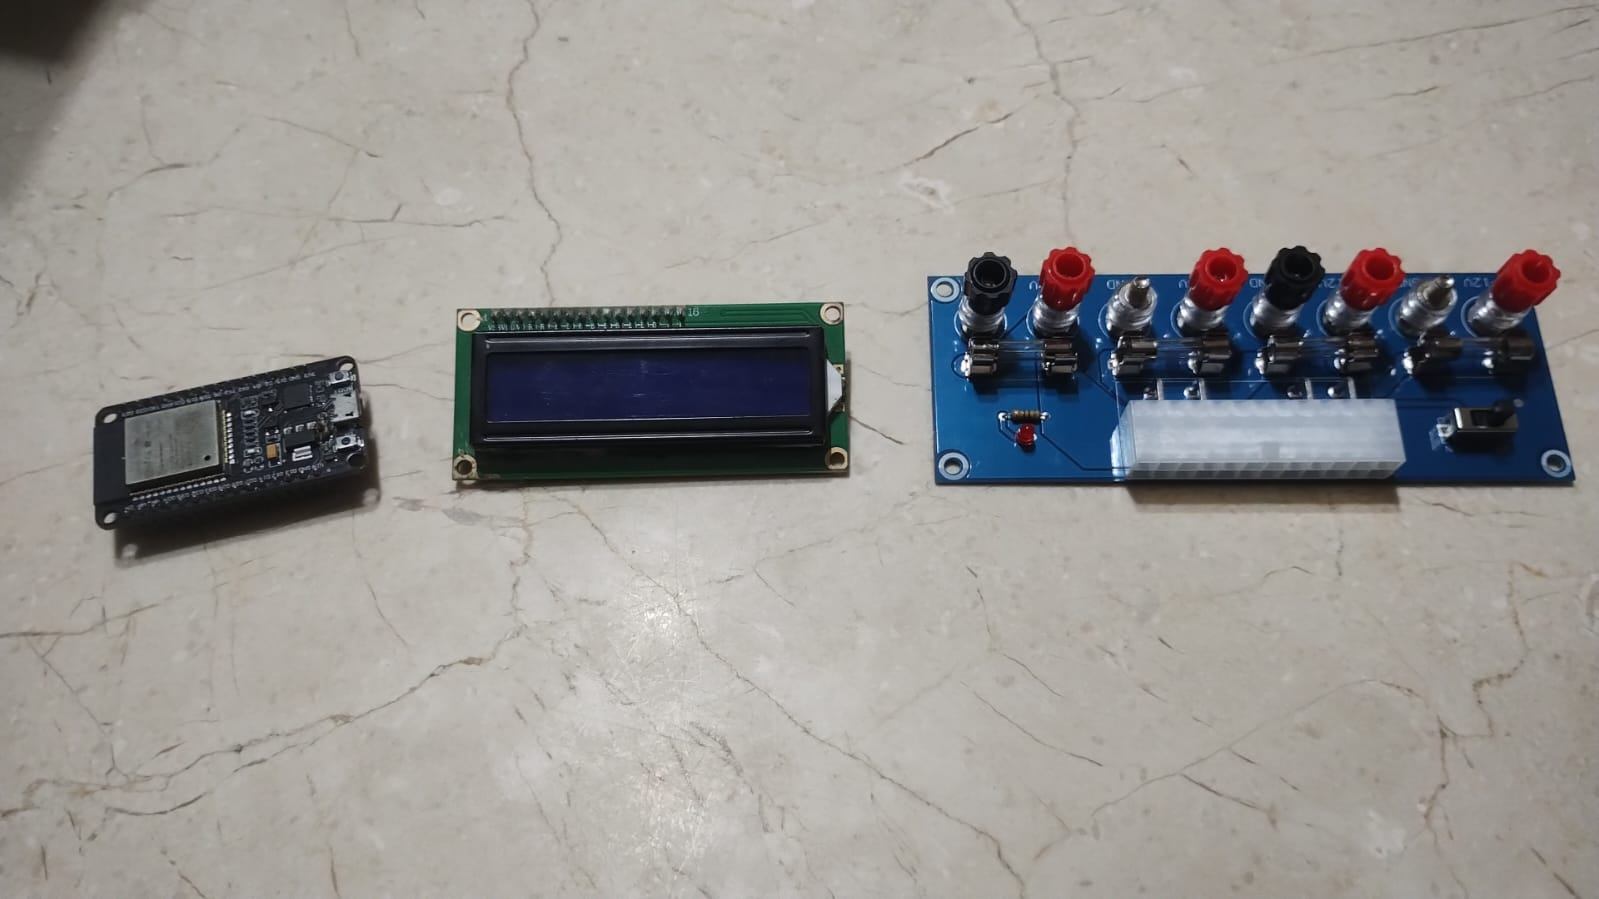
\includegraphics[width=0.8\textwidth]{figs/embarcados_peças.jpeg}
    \caption{Componentes parte do sistema embarcado, sendo o ESP32 (esquerda), display de LCD (centro), e adaptador de fonte 24 pinos de computador (direita).}
    \caption*{Fonte: Autor(2026)}
    \label{fig:embarcados_pecas}
\end{figure}

A arquitetura do sistema foi desenvolvida aproveitando a estrutura dual-core do ESP32, permitindo o processamento paralelo de tarefas por meio do FreeRTOS (Real-Time Operating System).
Esse sistema operacional em tempo real e de código aberto permite a divisão do programa em tarefas independentes, alocadas em cada um dos núcleos do microcontrolador.
A carga de trabalho do projeto está dividida da seguinte maneira: o núcleo 0 (vindo da contagem a partir da base 0) é responsável por toda a interface de comunicação, sendo essas o controle do servidor TCP e a interface com o LCD, enquando o núcleo 1 é responsável pelo controle do motor e do filtro $\alpha-\beta-\gamma$ embarcado.
Dessa forma, essa arquitetura garante um processador esteja exclusivamente destinado ao controle das malhas do motor, evitando que interferências ou latências de comunicação afetem a estabilidade e a precisão do rotor.

\begin{figure}[h]
    \centering
    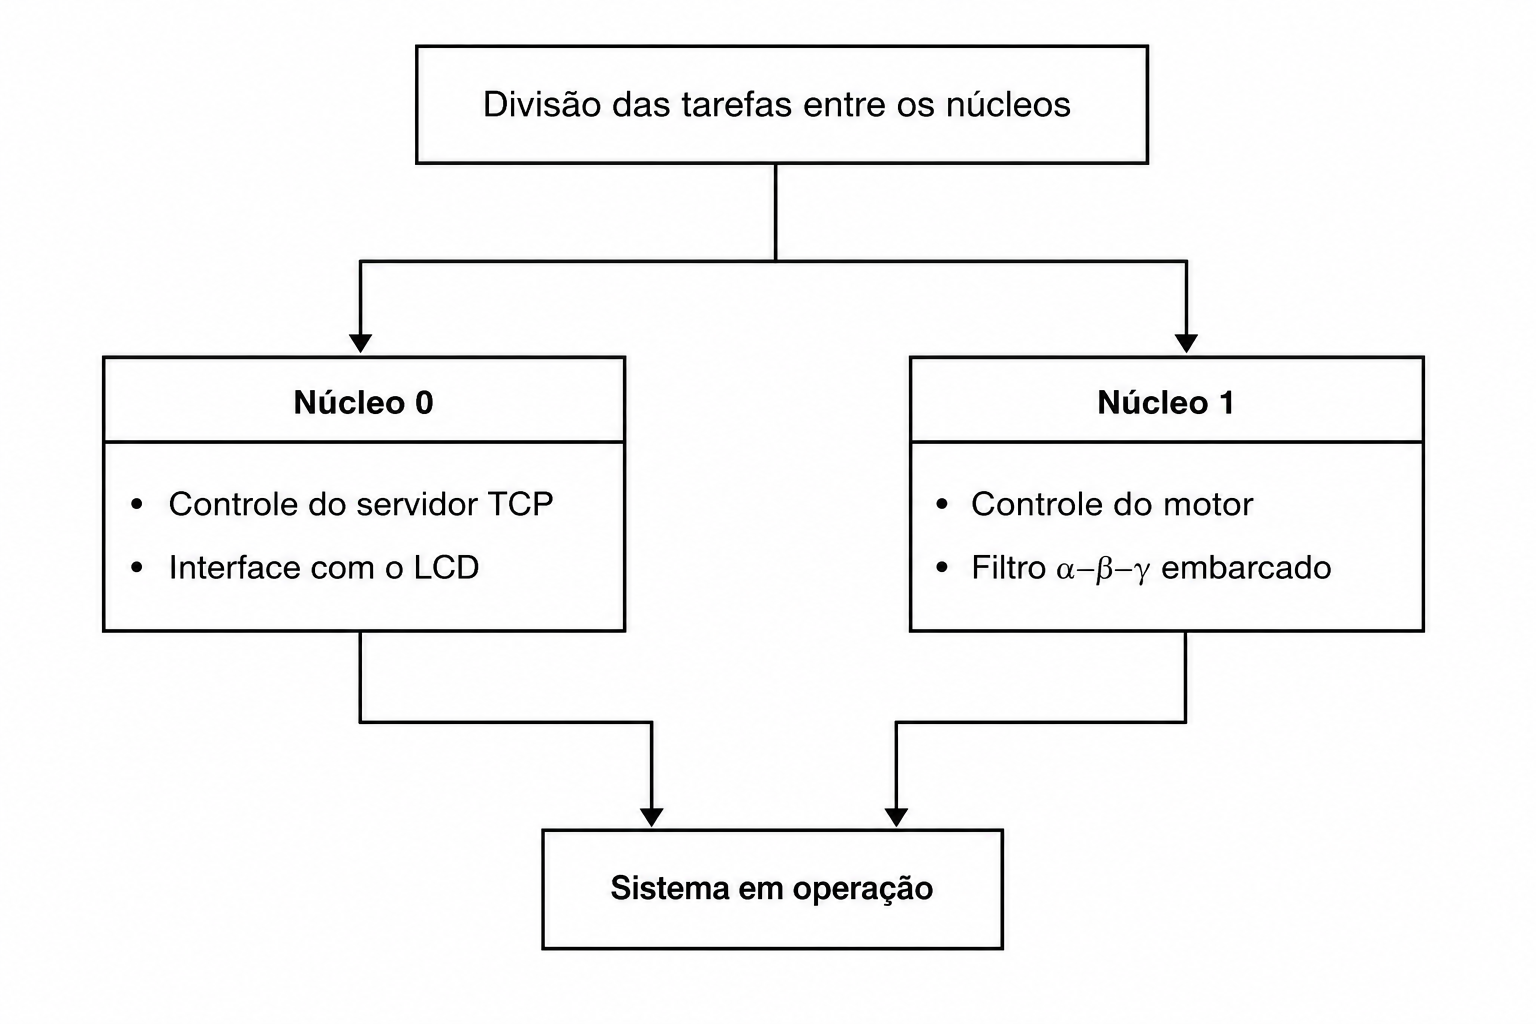
\includegraphics[width=0.8\textwidth]{figs/divisao_tarefas_nucleos_esp.png}
    \caption{Diagrama de divisão de tarefas entre os núcleos do microcontrolador.}
    \caption*{Fonte: Autor(2026)}
    \label{fig:divisao_tarefas_esp}
\end{figure}

\section{Implementação do Filtro Preditor}\label{sec:implementacao_filtro}
Para determinar os parâmetros do filtro preditor que será embarcado no processador, foram feitos alguns testes a partir de um servidor dummy (simulado) em um computador. Esse servidor era encarregado de receber todos os comandos enviados pelo software e catalogar as posições esperadas em diversos rastreios.
As capturas foram realizadas através de diversos dias, garantindo uma grande variação nas órbitas obtidas.
A partir desses dados, foi desenvolvido um algoritmo capaz de utilizar os valores dentro do limite de estabilidade discutido na seção \ref{sec:estimation} para encontrar o filtro cujos parâmetros geram o menor Erro Quadrático Médio (EQM ou MSE, na sigla em inglês).
Esse algoritmo altera os parâmetros alfa, beta e gama de acordo com um certo passo determinado e expõe todos os filtros aos mesmos dados, garantindo que a entrada não tenha um viés e os filtros estejam expostos às mesmas condições.
Com o Erro Quadrático Médio calculado para cada parâmetro, é possível estipular valores para o $\alpha$, $\beta$ e $\gamma$ que obtenha o melhor resultado preditivo de forma generalizada.
Deste modo, esses parâmetros calibrados foram embarcados na arquitetura do sistema apresentada na Seção \ref{sec:sistema_embarcado}.

\section{Controle de Velocidade e posição do Motor de Passo}\label{sec:controle_motor_passo}
A posição da estrutura é determinada de forma incremental a partir da posição inicial do motor, da relação de transmissão do sistema e da contagem dos pulsos emitidos pelo driver.
Embora o driver DRV8825 suporte frequências de pulso elevadas (de até aproximadamente 250 kHz), a resposta dinâmica dos motores de passo NEMA é mais restrita, limitando sua operação contínua a frequências na faixa de 1000 Hz.
Portanto, o controlador deve gerar sinal em uma frequência compatível com o motor, aproveitando a capacidade de micropasso (microstepping) do driver para aumentar a resolução e suavizar o deslocamento.
A partir dos valores de posição, velocidade e aceleração estimados pelo filtro $\alpha-\beta-\gamma$, o sistema calcula posições intermediárias preditas e determina as frequências de passo necessárias para realizar tal ação.
Essa interpolação reduz trancos na estrutura e garante um alinhamento mais estável e contínuo com o satélite.
Assim, com base na velocidade estimada pelo filtro, o controlador calcula a frequência de pulsos enviada ao DRV8825 para os eixos de azimute e elevação.
Para otimizar o tempo de processamento, é possível empregar equações simplificadas ou tabelas de consulta (lookup tables) pré-calculadas, ajustando a frequência e a resolução de passo necessárias para atingir a velocidade desejada em cada eixo.

\chapter{Resultados e Discussão}\label{cap:resultados}

\section{Estrutura do Pedestal}\label{sec:estrutura}
% O protótipo físico será baseado no mecanismo observado na figura \ref{fig:pedestal}. As peças utilizadas no modelo em 3D do pedestal são baseadas em materiais COTS (Commercial off-the-shelf, ou hardware comercial pronto para uso). Então, toda a geometria e os elementos são projetados para serem facilmente encontrados em lojas de materiais de construção.
% As polias utilizadas são GT2 de 20 e 40 dentes, com comprimento de cinto de \SI{10}{\milli\meter}. O cinto utilizado tem \SI{200}{\milli\meter} de comprimento, o que faz com que as distâncias entre centros das polias seja conhecida. Esses elementos são muito utilizados na confecção de impressoras 3D.
% Além das polias, os motores NEMA 17 são costumeiramentes utilizados em impressoas. Os drivers DRV8825 são altamente utilizados para controle de motores de passo, sendo facilmente encontrados em lojas de eletrônicos. O microcontrolador ESP 32 e o display de LCD podem ser encontrados tão facilmente quanto o restante dos componentes eletrônicos.
% O poste no qual o pedestal é dimensionado para utilizar uma viga de madeira de \SI{7,5}{\centi\meter} por \SI{7,5}{\centi\meter}, enquanto as dimensões da base são feitas para utilizar tábuas de \SI{0,9}{\centi\meter} por \SI{9,5}{\centi\meter}. O fio de cobre macisso utilizado para a confecção da antena foi obtido a partir de um cabo para aterramento de 7 fios, no qual cada fio individual possui o padrão \SI{10}{AWG}.
% Enquanto a tela de alumínio para o plano Terra foi obtida de uma tela mosquiteira de alumínio de \SI{1}{\meter\squared}. A chapa de alumínio que compõe o plano Terra é feita a partir de um rufo metálico para telhado. Dessa forma, os materiais são facilmente encontrados em lojas de materiais.

% A estrutura da antena foi confeccionada com o auxílio de uma impressora 3D, feita com PLA (ácido polilático). O resultado pode ser visto na figura \ref{fig:pecas_antena}. A baixa densidade do plástico unida com a densidade de material interna à peça (de 20\%) faz com que toda a estrutura da antena pese \SI{233}{\gram}.
% Unida com aproximadamente \SI{82}{\gram} de cobre para construir a antena, \SI{60}{\gram} da chapa de plano Terra, e \SI{225}{\gram} da tela para fazer o cone, o peso final total da estrutura é de aproximadame \SI{600}{\gram}. Dessa forma, essa antena é ideal para operar com os motores descritos na seção \ref{sec:motor_passo}.
% Esse refinamento da antena faz com que haja uma grande compatibilidade com o restante do sistema.

O protótipo físico será baseado no mecanismo apresentado na Figura~\ref{fig:pedestal}. As peças utilizadas no modelo 3D do pedestal empregam componentes COTS (\textit{Commercial Off-The-Shelf}, ou seja, hardware comercial pronto para uso). Dessa forma, a geometria e os elementos foram projetados para utilizar materiais de fácil acesso no comércio local e em lojas de construção.

As polias utilizadas são do tipo GT2, de 20 e 40 dentes, associadas a uma correia dentada de \SI{10}{\milli\meter} de largura e \SI{200}{\milli\meter} de comprimento perimetral, o que estabelece uma distância entre centros conhecida. Esses elementos, assim como os motores de passo NEMA 17, são amplamente empregados na fabricação de impressoras 3D.

Para o acionamento dos motores, foram adotados os drivers DRV8825, comumente encontrados em lojas de eletrônica. O microcontrolador ESP32 e o display LCD seguem a mesma facilidade de aquisição do restante dos componentes eletrônicos.

A estrutura do poste foi dimensionada para utilizar um pontalete de madeira de \SI{7,5}{\centi\meter} $\times$ \SI{7,5}{\centi\meter}, enquanto a base foi projetada para tábuas de \SI{0,9}{\centi\meter} $\times$ \SI{9,5}{\centi\meter}. O fio de cobre maciço usado para a confecção da antena foi obtido a partir do desmembramento de um cabo de aterramento de 7 vias, no qual cada condutor individual possui bitola \SI{10}{AWG}.

A tela de alumínio empregada no plano de terra foi adaptada de uma tela mosquiteira de alumínio de \SI{1}{\square\meter}. Já a chapa metálica complementar do plano de terra foi produzida a partir de um rufo para telhado.

A estrutura de suporte da antena foi confeccionada via impressão 3D em PLA (ácido polilático), conforme ilustrado na Figura~\ref{fig:pecas_antena}. A baixa densidade do polímero somada ao preenchimento interno (\textit{infill}) de \SI{20}{\percent} resultou em uma massa de \SI{233}{\gram} para a estrutura plástica da antena.

Somando-se aproximadamente \SI{82}{\gram} de cobre para a fiação, \SI{60}{\gram} da chapa e \SI{225}{\gram} da tela de alumínio, a estrutura completa da antena apresenta uma massa total de aproximadamente \SI{600}{\gram}. Essa massa reduzida torna o conjunto adequado para a operação com os motores especificados na Seção~\ref{sec:motor_passo}, garantindo a compatibilidade mecânica do sistema.
\section{Levantamento dos Parâmetros do Filtro $\alpha-\beta-\gamma$}

Conforme apresentado na Seção~\ref{sec:implementacao_filtro}, os parâmetros iniciais do filtro foram obtidos a partir de dados de rastreamento de diversos satélites de órbita baixa (LEO). 
Em seguida, aplicou-se um método computacional de varredura sistemática (\textit{grid search}) para a otimização dos coeficientes, variando-se os parâmetros em incrementos de $0,1$ para $\alpha$ e $\beta$, e de $0,01$ para $\gamma$, respeitando estritamente os limites de estabilidade definidos pelo Critério de Jury (Seção~\ref{sec:estimation}).

O desempenho do filtro para cada combinação de parâmetros foi avaliado ao longo das passagens dos satélites por meio do Erro Quadrático Médio (EQM). A partir desses resultados, geraram-se superfícies tridimensionais correlacionando os coeficientes ao menor erro obtido. 
Essa representação permitiu identificar uma região operacional ótima, na qual o filtro $\alpha-\beta-\gamma$ apresenta convergência satisfatória para a maioria das trajetórias orbitais analisadas.

\begin{figure}[htbp]
    \centering
    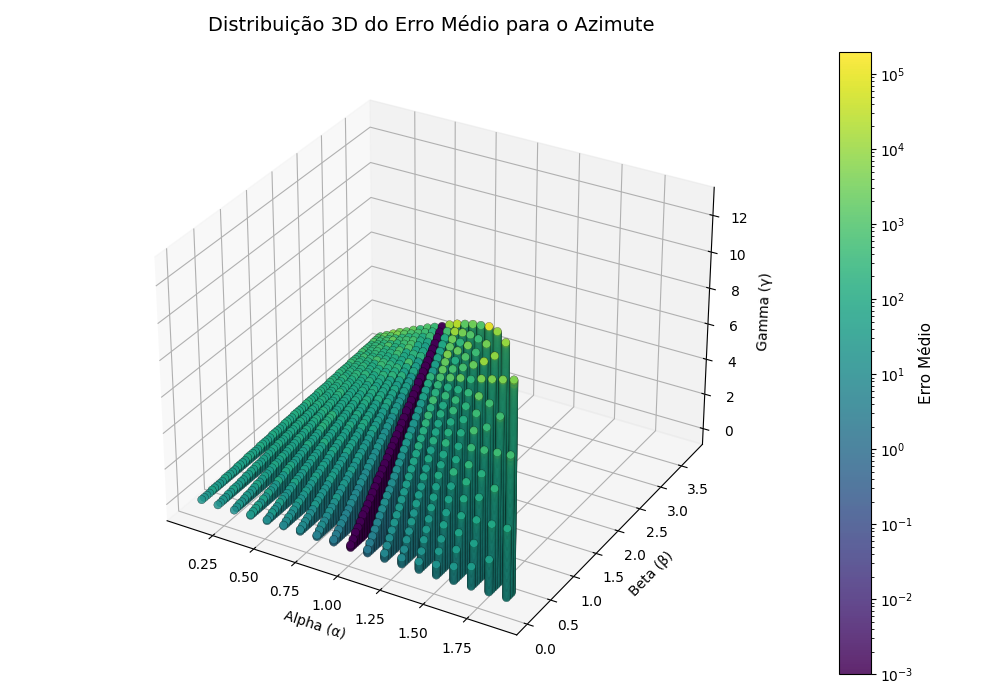
\includegraphics[width=0.8\textwidth]{figs/Plot_alfa_beta_gamma_az.png}
    \caption{Superfície de desempenho dos parâmetros $\alpha$, $\beta$ e $\gamma$ para o eixo de azimute.}
    \caption*{Fonte: Autor (2026)}
    \label{fig:param_az}
\end{figure}

\begin{figure}[htbp]
    \centering
    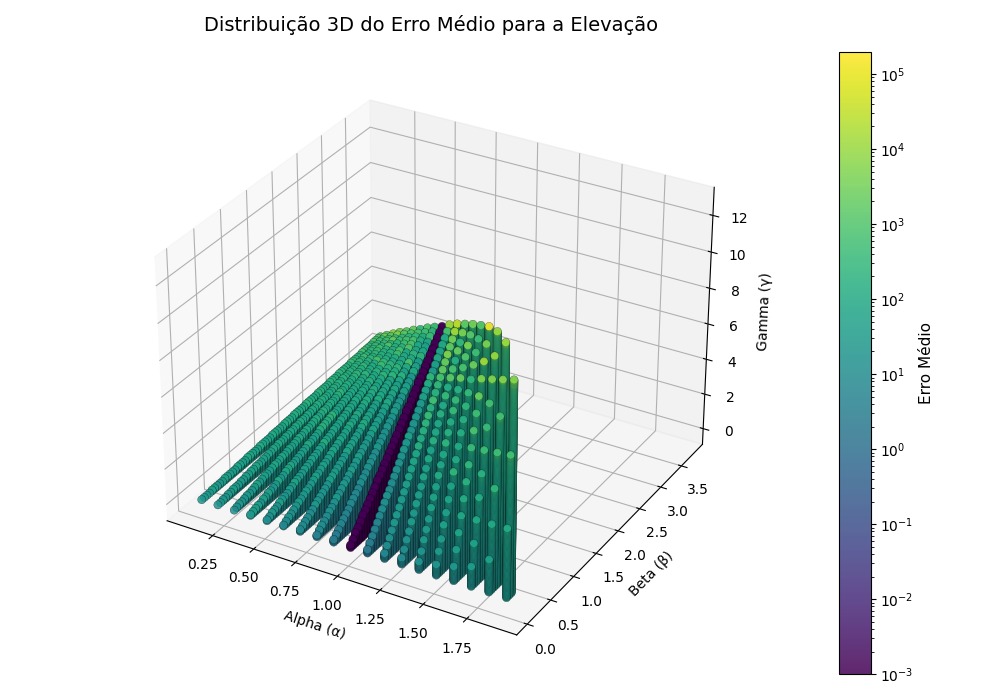
\includegraphics[width=0.8\textwidth]{figs/Plot_alfa_beta_gamma_el.png}
    \caption{Superfície de desempenho dos parâmetros $\alpha$, $\beta$ e $\gamma$ para o eixo de elevação.}
    \caption*{Fonte: Autor (2026)}
    \label{fig:param_el}
\end{figure}

A partir dessa análise, definiram-se os parâmetros do filtro embarcado como $\alpha = 1{,}00$, $\beta = 0{,}05$ e $\gamma = 0{,}00$. Observa-se claramente a existência de uma região onde valores reduzidos de $\beta$ minimizam o erro de estimação. 
Esse comportamento evidencia que a informação orbital fornecida pelo software permite manter a precisão do rastreamento da posição do satélite ao longo da trajetória, sem a introdução de ruídos perceptíveis.

Consequentemente, uma vez estabelecida a estimativa inicial de velocidade do alvo pelo sistema, esta sofrerá apenas variações marginais durante o rastreio. 
Essa característica confere robustez ao pedestal, permitindo que ele continue acompanhando a trajetória do satélite por um período prolongado, mesmo na ocorrência de eventuais interrupções temporárias na comunicação com o software de controle.
\chapter{Conclusão e Trabalhos Futuros}

O presente trabalho apresentou o projeto, a modelagem, a implementação e a validação experimental de um protótipo automatizado de pedestal bi-axial (azimute e elevação) integrado a uma antena helicone para o rastreio automático de satélites em órbita terrestre baixa (LEO) e recepção de sinais meteorológicos no padrão HRPT na faixa de 1,7~GHz.

A modelagem cinemática direta do mecanismo bi-axial, formulada rigorosamente por meio da convenção dos parâmetros de Denavit-Hartenberg (D-H), forneceu a base geométrica para o cálculo das matrizes de transformação homogênea, assegurando o correto apontamento angular da antena ao longo de toda a semiesfera do horizonte local.

No âmbito dos sistemas embarcados e de controle, a arquitetura dual-core do microcontrolador ESP32 sob a gerência do sistema operacional em tempo real FreeRTOS demonstrou elevada eficiência. A segregação estruturada do processamento — alocando o servidor de comunicação TCP e a interface de telemetria LCD no Núcleo 0, enquanto o Núcleo 1 executou exclusivamente as malhas de controle dos motores de passo NEMA 17 (via drivers DRV8825 em micropasso) e o algoritmo do filtro preditivo $\alpha-\beta-\gamma$ — eliminou latências de comunicação e preveniu flutuações no tempo de amostragem do controle.

Para garantir a suavidade e a continuidade da trajetória sem comprometer a capacidade computacional do sistema embarcado, implementou-se o filtro preditivo de terceira ordem $\alpha-\beta-\gamma$. A sintonia otimizada dos coeficientes via varredura sistemática (\textit{grid search}), balizada pelos limites do Critério de Estabilidade de Jury e avaliada pelo Erro Quadrático Médio (EQM), resultou no conjunto de parâmetros calibrados $\alpha = 1{,}00$, $\beta = 0{,}05$ e $\gamma = 0{,}00$.

A convergência observada do ganho de velocidade $\beta$ para um patamar estritamente reduzido ($\beta \approx 0{,}05$) e do ganho de aceleração $\gamma$ para zero justifica-se teórica e empiricamente por três fatores determinantes:
\begin{enumerate}
    \item \textbf{Atenuação da Propagação de Ruído:} A atualização do estado de velocidade no filtro $\alpha-\beta-\gamma$ envolve a divisão pelo período de amostragem ($\frac{\beta}{T}$). Valorações mais elevadas de $\beta$ provocam a amplificação do ruído de medição proveniente das estimativas angulares, introduzindo derivadas espúrias que desestabilizam o acionamento dos motores.
    \item \textbf{Consistência e Previsibilidade Orbital:} Uma vez que as posições orbitais fornecidas pelo software de rastreio (SatDump via TLE/Keplerianos) apresentam elevada acurácia determinística ao longo do tempo, a dinâmica de variação de velocidade é adequadamente sustentada pela equação de propagação do modelo preditivo, reduzindo a necessidade de correções derivativas agressivas baseadas no termo de inovação.
    \item \textbf{Estabilidade e Alocação de Polos:} A análise de estabilidade em tempo discreto via teste de Jury confirma que o aumento simultâneo dos ganhos $\beta$ e $\gamma$ desloca os autovalores da matriz de transição do filtro em malha fechada para fora do círculo unitário no plano $z$, resultando em instabilidade e divergência do erro de estimativa.
\end{enumerate}

No subsistema de radiofrequência, a antena helicone desenvolvida em estrutura impressa em PLA e malha de alumínio (com massa total de aproximadamente 600~g) operou em regime de modo axial compatível com a polarização circular à direita (RHCP). Associada ao estágio pré-amplificador e filtro SAW (Nooelec SAWBird+ GOES) e ao receptor SDR (RTL-SDR V4), a estação em solo comprovou viabilidade técnica ao estabelecer enlaces estáveis de RF e viabilizar a recepção de telemetria sem perdas de desalinhamento angular.

Em suma, os objetivos propostos foram plenamente alcançados, resultando em um sistema de alinhamento e rastreio de baixo custo, estruturalmente leve, estável e computacionalmente eficiente.

\section*{Trabalhos Futuros}

Como continuidade deste trabalho e visando o aprimoramento do protótipo, sugerem-se as seguintes linhas de pesquisa e desenvolvimento:

\begin{itemize}
    \item \textbf{Filtro Adaptativo de Ganhos:} Implementar uma estrutura de filtragem $\alpha-\beta-\gamma$ adaptativa, capaz de ajustar os coeficientes $\beta$ e $\gamma$ em tempo real apenas durante a detecção de manobras com elevada aceleração angular (como no momento de culminação do satélite próximo ao Zênite), mantendo os ganhos atenuados durante o regime permanente.
    \item \textbf{Feedback de Posição em Malha Fechada:} Incorporar encoders absolutos de alta resolução nos eixos de azimute e elevação para proporcionar malha fechada de posição direta na estrutura mecânica, mitigando eventuais perdas de passos dos motores sob torque de carga externa ou ventos.
    \item \textbf{Rastreio Autônomo por Sinal de RF (\textit{Closed-loop Autotrack}):} Desenvolver um algoritmo de alinhamento fino baseado no indicador de intensidade do sinal recebido (RSSI) ou técnica monopulso, permitindo que a antena corrija pequenos desvios de apontamento de forma autônoma a partir da máxima potência de RF capturada pelo receptor SDR.
    \item \textbf{Aprimoramento Mecânico e Proteção Ambiental:} Evoluir a estrutura do pedestal para ligas metálicas leves (ou polímeros de grau engenharia) com cúpula de proteção (\textit{radome}), permitindo a operação contínua do sistema em ambientes externos sujeitos a intempéries atmosféricas.
\end{itemize}

% PARTE - Define a divisão do documento em partes (Não é obrigatório)
%\part{Preparação da pesquisa}
%\input{capitulos/referencias}
%\input{capitulos/ferramentas}

% PARTE
%\part{Proposta}
%\input{capitulos/proposta}

% PARTE
%\part{Parte Final}
%\chapter{Resultados e Discussão}\label{cap:resultados}

\section{Estrutura do Pedestal}\label{sec:estrutura}
% O protótipo físico será baseado no mecanismo observado na figura \ref{fig:pedestal}. As peças utilizadas no modelo em 3D do pedestal são baseadas em materiais COTS (Commercial off-the-shelf, ou hardware comercial pronto para uso). Então, toda a geometria e os elementos são projetados para serem facilmente encontrados em lojas de materiais de construção.
% As polias utilizadas são GT2 de 20 e 40 dentes, com comprimento de cinto de \SI{10}{\milli\meter}. O cinto utilizado tem \SI{200}{\milli\meter} de comprimento, o que faz com que as distâncias entre centros das polias seja conhecida. Esses elementos são muito utilizados na confecção de impressoras 3D.
% Além das polias, os motores NEMA 17 são costumeiramentes utilizados em impressoas. Os drivers DRV8825 são altamente utilizados para controle de motores de passo, sendo facilmente encontrados em lojas de eletrônicos. O microcontrolador ESP 32 e o display de LCD podem ser encontrados tão facilmente quanto o restante dos componentes eletrônicos.
% O poste no qual o pedestal é dimensionado para utilizar uma viga de madeira de \SI{7,5}{\centi\meter} por \SI{7,5}{\centi\meter}, enquanto as dimensões da base são feitas para utilizar tábuas de \SI{0,9}{\centi\meter} por \SI{9,5}{\centi\meter}. O fio de cobre macisso utilizado para a confecção da antena foi obtido a partir de um cabo para aterramento de 7 fios, no qual cada fio individual possui o padrão \SI{10}{AWG}.
% Enquanto a tela de alumínio para o plano Terra foi obtida de uma tela mosquiteira de alumínio de \SI{1}{\meter\squared}. A chapa de alumínio que compõe o plano Terra é feita a partir de um rufo metálico para telhado. Dessa forma, os materiais são facilmente encontrados em lojas de materiais.

% A estrutura da antena foi confeccionada com o auxílio de uma impressora 3D, feita com PLA (ácido polilático). O resultado pode ser visto na figura \ref{fig:pecas_antena}. A baixa densidade do plástico unida com a densidade de material interna à peça (de 20\%) faz com que toda a estrutura da antena pese \SI{233}{\gram}.
% Unida com aproximadamente \SI{82}{\gram} de cobre para construir a antena, \SI{60}{\gram} da chapa de plano Terra, e \SI{225}{\gram} da tela para fazer o cone, o peso final total da estrutura é de aproximadame \SI{600}{\gram}. Dessa forma, essa antena é ideal para operar com os motores descritos na seção \ref{sec:motor_passo}.
% Esse refinamento da antena faz com que haja uma grande compatibilidade com o restante do sistema.

O protótipo físico será baseado no mecanismo apresentado na Figura~\ref{fig:pedestal}. As peças utilizadas no modelo 3D do pedestal empregam componentes COTS (\textit{Commercial Off-The-Shelf}, ou seja, hardware comercial pronto para uso). Dessa forma, a geometria e os elementos foram projetados para utilizar materiais de fácil acesso no comércio local e em lojas de construção.

As polias utilizadas são do tipo GT2, de 20 e 40 dentes, associadas a uma correia dentada de \SI{10}{\milli\meter} de largura e \SI{200}{\milli\meter} de comprimento perimetral, o que estabelece uma distância entre centros conhecida. Esses elementos, assim como os motores de passo NEMA 17, são amplamente empregados na fabricação de impressoras 3D.

Para o acionamento dos motores, foram adotados os drivers DRV8825, comumente encontrados em lojas de eletrônica. O microcontrolador ESP32 e o display LCD seguem a mesma facilidade de aquisição do restante dos componentes eletrônicos.

A estrutura do poste foi dimensionada para utilizar um pontalete de madeira de \SI{7,5}{\centi\meter} $\times$ \SI{7,5}{\centi\meter}, enquanto a base foi projetada para tábuas de \SI{0,9}{\centi\meter} $\times$ \SI{9,5}{\centi\meter}. O fio de cobre maciço usado para a confecção da antena foi obtido a partir do desmembramento de um cabo de aterramento de 7 vias, no qual cada condutor individual possui bitola \SI{10}{AWG}.

A tela de alumínio empregada no plano de terra foi adaptada de uma tela mosquiteira de alumínio de \SI{1}{\square\meter}. Já a chapa metálica complementar do plano de terra foi produzida a partir de um rufo para telhado.

A estrutura de suporte da antena foi confeccionada via impressão 3D em PLA (ácido polilático), conforme ilustrado na Figura~\ref{fig:pecas_antena}. A baixa densidade do polímero somada ao preenchimento interno (\textit{infill}) de \SI{20}{\percent} resultou em uma massa de \SI{233}{\gram} para a estrutura plástica da antena.

Somando-se aproximadamente \SI{82}{\gram} de cobre para a fiação, \SI{60}{\gram} da chapa e \SI{225}{\gram} da tela de alumínio, a estrutura completa da antena apresenta uma massa total de aproximadamente \SI{600}{\gram}. Essa massa reduzida torna o conjunto adequado para a operação com os motores especificados na Seção~\ref{sec:motor_passo}, garantindo a compatibilidade mecânica do sistema.
\section{Levantamento dos Parâmetros do Filtro $\alpha-\beta-\gamma$}

Conforme apresentado na Seção~\ref{sec:implementacao_filtro}, os parâmetros iniciais do filtro foram obtidos a partir de dados de rastreamento de diversos satélites de órbita baixa (LEO). 
Em seguida, aplicou-se um método computacional de varredura sistemática (\textit{grid search}) para a otimização dos coeficientes, variando-se os parâmetros em incrementos de $0,1$ para $\alpha$ e $\beta$, e de $0,01$ para $\gamma$, respeitando estritamente os limites de estabilidade definidos pelo Critério de Jury (Seção~\ref{sec:estimation}).

O desempenho do filtro para cada combinação de parâmetros foi avaliado ao longo das passagens dos satélites por meio do Erro Quadrático Médio (EQM). A partir desses resultados, geraram-se superfícies tridimensionais correlacionando os coeficientes ao menor erro obtido. 
Essa representação permitiu identificar uma região operacional ótima, na qual o filtro $\alpha-\beta-\gamma$ apresenta convergência satisfatória para a maioria das trajetórias orbitais analisadas.

\begin{figure}[htbp]
    \centering
    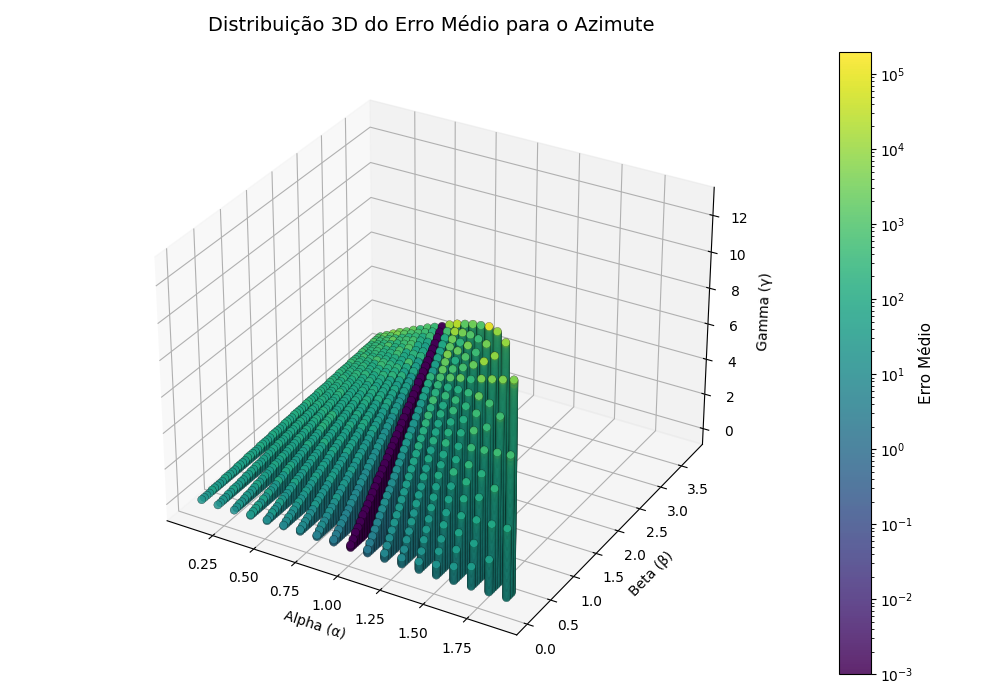
\includegraphics[width=0.8\textwidth]{figs/Plot_alfa_beta_gamma_az.png}
    \caption{Superfície de desempenho dos parâmetros $\alpha$, $\beta$ e $\gamma$ para o eixo de azimute.}
    \caption*{Fonte: Autor (2026)}
    \label{fig:param_az}
\end{figure}

\begin{figure}[htbp]
    \centering
    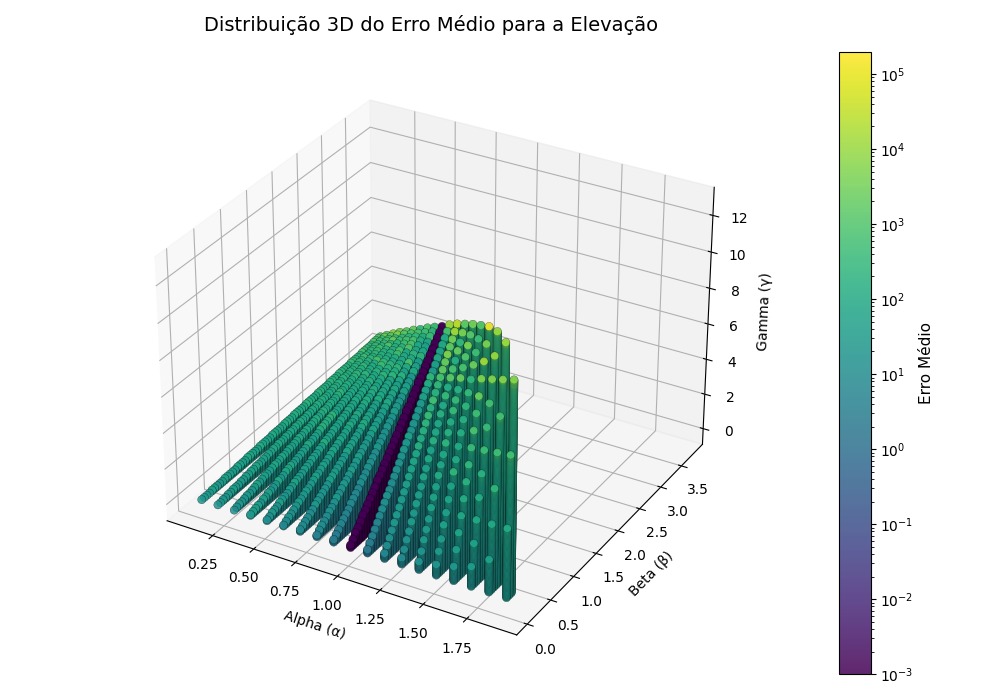
\includegraphics[width=0.8\textwidth]{figs/Plot_alfa_beta_gamma_el.png}
    \caption{Superfície de desempenho dos parâmetros $\alpha$, $\beta$ e $\gamma$ para o eixo de elevação.}
    \caption*{Fonte: Autor (2026)}
    \label{fig:param_el}
\end{figure}

A partir dessa análise, definiram-se os parâmetros do filtro embarcado como $\alpha = 1{,}00$, $\beta = 0{,}05$ e $\gamma = 0{,}00$. Observa-se claramente a existência de uma região onde valores reduzidos de $\beta$ minimizam o erro de estimação. 
Esse comportamento evidencia que a informação orbital fornecida pelo software permite manter a precisão do rastreamento da posição do satélite ao longo da trajetória, sem a introdução de ruídos perceptíveis.

Consequentemente, uma vez estabelecida a estimativa inicial de velocidade do alvo pelo sistema, esta sofrerá apenas variações marginais durante o rastreio. 
Essa característica confere robustez ao pedestal, permitindo que ele continue acompanhando a trajetória do satélite por um período prolongado, mesmo na ocorrência de eventuais interrupções temporárias na comunicação com o software de controle.
% \chapter{Conclusão e Trabalhos Futuros}

O presente trabalho apresentou o projeto, a modelagem, a implementação e a validação experimental de um protótipo automatizado de pedestal bi-axial (azimute e elevação) integrado a uma antena helicone para o rastreio automático de satélites em órbita terrestre baixa (LEO) e recepção de sinais meteorológicos no padrão HRPT na faixa de 1,7~GHz.

A modelagem cinemática direta do mecanismo bi-axial, formulada rigorosamente por meio da convenção dos parâmetros de Denavit-Hartenberg (D-H), forneceu a base geométrica para o cálculo das matrizes de transformação homogênea, assegurando o correto apontamento angular da antena ao longo de toda a semiesfera do horizonte local.

No âmbito dos sistemas embarcados e de controle, a arquitetura dual-core do microcontrolador ESP32 sob a gerência do sistema operacional em tempo real FreeRTOS demonstrou elevada eficiência. A segregação estruturada do processamento — alocando o servidor de comunicação TCP e a interface de telemetria LCD no Núcleo 0, enquanto o Núcleo 1 executou exclusivamente as malhas de controle dos motores de passo NEMA 17 (via drivers DRV8825 em micropasso) e o algoritmo do filtro preditivo $\alpha-\beta-\gamma$ — eliminou latências de comunicação e preveniu flutuações no tempo de amostragem do controle.

Para garantir a suavidade e a continuidade da trajetória sem comprometer a capacidade computacional do sistema embarcado, implementou-se o filtro preditivo de terceira ordem $\alpha-\beta-\gamma$. A sintonia otimizada dos coeficientes via varredura sistemática (\textit{grid search}), balizada pelos limites do Critério de Estabilidade de Jury e avaliada pelo Erro Quadrático Médio (EQM), resultou no conjunto de parâmetros calibrados $\alpha = 1{,}00$, $\beta = 0{,}05$ e $\gamma = 0{,}00$.

A convergência observada do ganho de velocidade $\beta$ para um patamar estritamente reduzido ($\beta \approx 0{,}05$) e do ganho de aceleração $\gamma$ para zero justifica-se teórica e empiricamente por três fatores determinantes:
\begin{enumerate}
    \item \textbf{Atenuação da Propagação de Ruído:} A atualização do estado de velocidade no filtro $\alpha-\beta-\gamma$ envolve a divisão pelo período de amostragem ($\frac{\beta}{T}$). Valorações mais elevadas de $\beta$ provocam a amplificação do ruído de medição proveniente das estimativas angulares, introduzindo derivadas espúrias que desestabilizam o acionamento dos motores.
    \item \textbf{Consistência e Previsibilidade Orbital:} Uma vez que as posições orbitais fornecidas pelo software de rastreio (SatDump via TLE/Keplerianos) apresentam elevada acurácia determinística ao longo do tempo, a dinâmica de variação de velocidade é adequadamente sustentada pela equação de propagação do modelo preditivo, reduzindo a necessidade de correções derivativas agressivas baseadas no termo de inovação.
    \item \textbf{Estabilidade e Alocação de Polos:} A análise de estabilidade em tempo discreto via teste de Jury confirma que o aumento simultâneo dos ganhos $\beta$ e $\gamma$ desloca os autovalores da matriz de transição do filtro em malha fechada para fora do círculo unitário no plano $z$, resultando em instabilidade e divergência do erro de estimativa.
\end{enumerate}

No subsistema de radiofrequência, a antena helicone desenvolvida em estrutura impressa em PLA e malha de alumínio (com massa total de aproximadamente 600~g) operou em regime de modo axial compatível com a polarização circular à direita (RHCP). Associada ao estágio pré-amplificador e filtro SAW (Nooelec SAWBird+ GOES) e ao receptor SDR (RTL-SDR V4), a estação em solo comprovou viabilidade técnica ao estabelecer enlaces estáveis de RF e viabilizar a recepção de telemetria sem perdas de desalinhamento angular.

Em suma, os objetivos propostos foram plenamente alcançados, resultando em um sistema de alinhamento e rastreio de baixo custo, estruturalmente leve, estável e computacionalmente eficiente.

\section*{Trabalhos Futuros}

Como continuidade deste trabalho e visando o aprimoramento do protótipo, sugerem-se as seguintes linhas de pesquisa e desenvolvimento:

\begin{itemize}
    \item \textbf{Filtro Adaptativo de Ganhos:} Implementar uma estrutura de filtragem $\alpha-\beta-\gamma$ adaptativa, capaz de ajustar os coeficientes $\beta$ e $\gamma$ em tempo real apenas durante a detecção de manobras com elevada aceleração angular (como no momento de culminação do satélite próximo ao Zênite), mantendo os ganhos atenuados durante o regime permanente.
    \item \textbf{Feedback de Posição em Malha Fechada:} Incorporar encoders absolutos de alta resolução nos eixos de azimute e elevação para proporcionar malha fechada de posição direta na estrutura mecânica, mitigando eventuais perdas de passos dos motores sob torque de carga externa ou ventos.
    \item \textbf{Rastreio Autônomo por Sinal de RF (\textit{Closed-loop Autotrack}):} Desenvolver um algoritmo de alinhamento fino baseado no indicador de intensidade do sinal recebido (RSSI) ou técnica monopulso, permitindo que a antena corrija pequenos desvios de apontamento de forma autônoma a partir da máxima potência de RF capturada pelo receptor SDR.
    \item \textbf{Aprimoramento Mecânico e Proteção Ambiental:} Evoluir a estrutura do pedestal para ligas metálicas leves (ou polímeros de grau engenharia) com cúpula de proteção (\textit{radome}), permitindo a operação contínua do sistema em ambientes externos sujeitos a intempéries atmosféricas.
\end{itemize}

% ----------------------------------------------------------
% ELEMENTOS PÓS-TEXTUAIS (Referências, Glossário, Apêndices)
% ----------------------------------------------------------
\postextual

% Referências bibliográficas
% \bibliographystyle{ieeetran}
% \bibliography{bibliografia}
\printbibliography

% Glossário (Consulte o manual)
%\glossary

% Apêndices
% \input{postextual/apendices}

% Anexos
% \input{postextual/anexos}

% Índice remissivo (Consultar manual)
%\phantompart
%\printindex

\end{document}
